\documentclass[10pt, a4paper]{article} %twocolumn
\usepackage{graphicx}
\usepackage{xcolor}
\usepackage{enumitem}
\usepackage{hyperref}
\usepackage{wrapfig}
\usepackage{lipsum}
\usepackage{caption}
\usepackage{subcaption}
\usepackage{float}
\usepackage[numbers]{natbib}
\usepackage{algorithm}
\usepackage{algpseudocode}
\usepackage{listings}

\hypersetup{
colorlinks=true,
linkcolor=blue,
urlcolor=teal,
citecolor=blue
}

\title{Saklain Hasan 2}
\author{Saklain Hasan}
\date{June 2026}

\begin{document}

\maketitle

\tableofcontents
\definecolor{customercol1}{RGB}{123,9,23}

\section{Text Formatting}

This is example of a colored text. \textcolor{red}{this is a red text}. Tis is using a \textcolor{customercol1}{custom color}.
tintin 

\section{Nested and Mixed List}

\begin{enumerate}[label=(\alph*)]
    \item System setup
    \item Simulation Steps
    \begin{enumerate}
        \item item A
        \item item B
    \end{enumerate}
\end{enumerate}


\begin{enumerate}
    \item[!] item A
    \item[.] item B
\end{enumerate}

\newpage

\section{Image and Float placement}

\begin{figure}[ht]
    \centering
    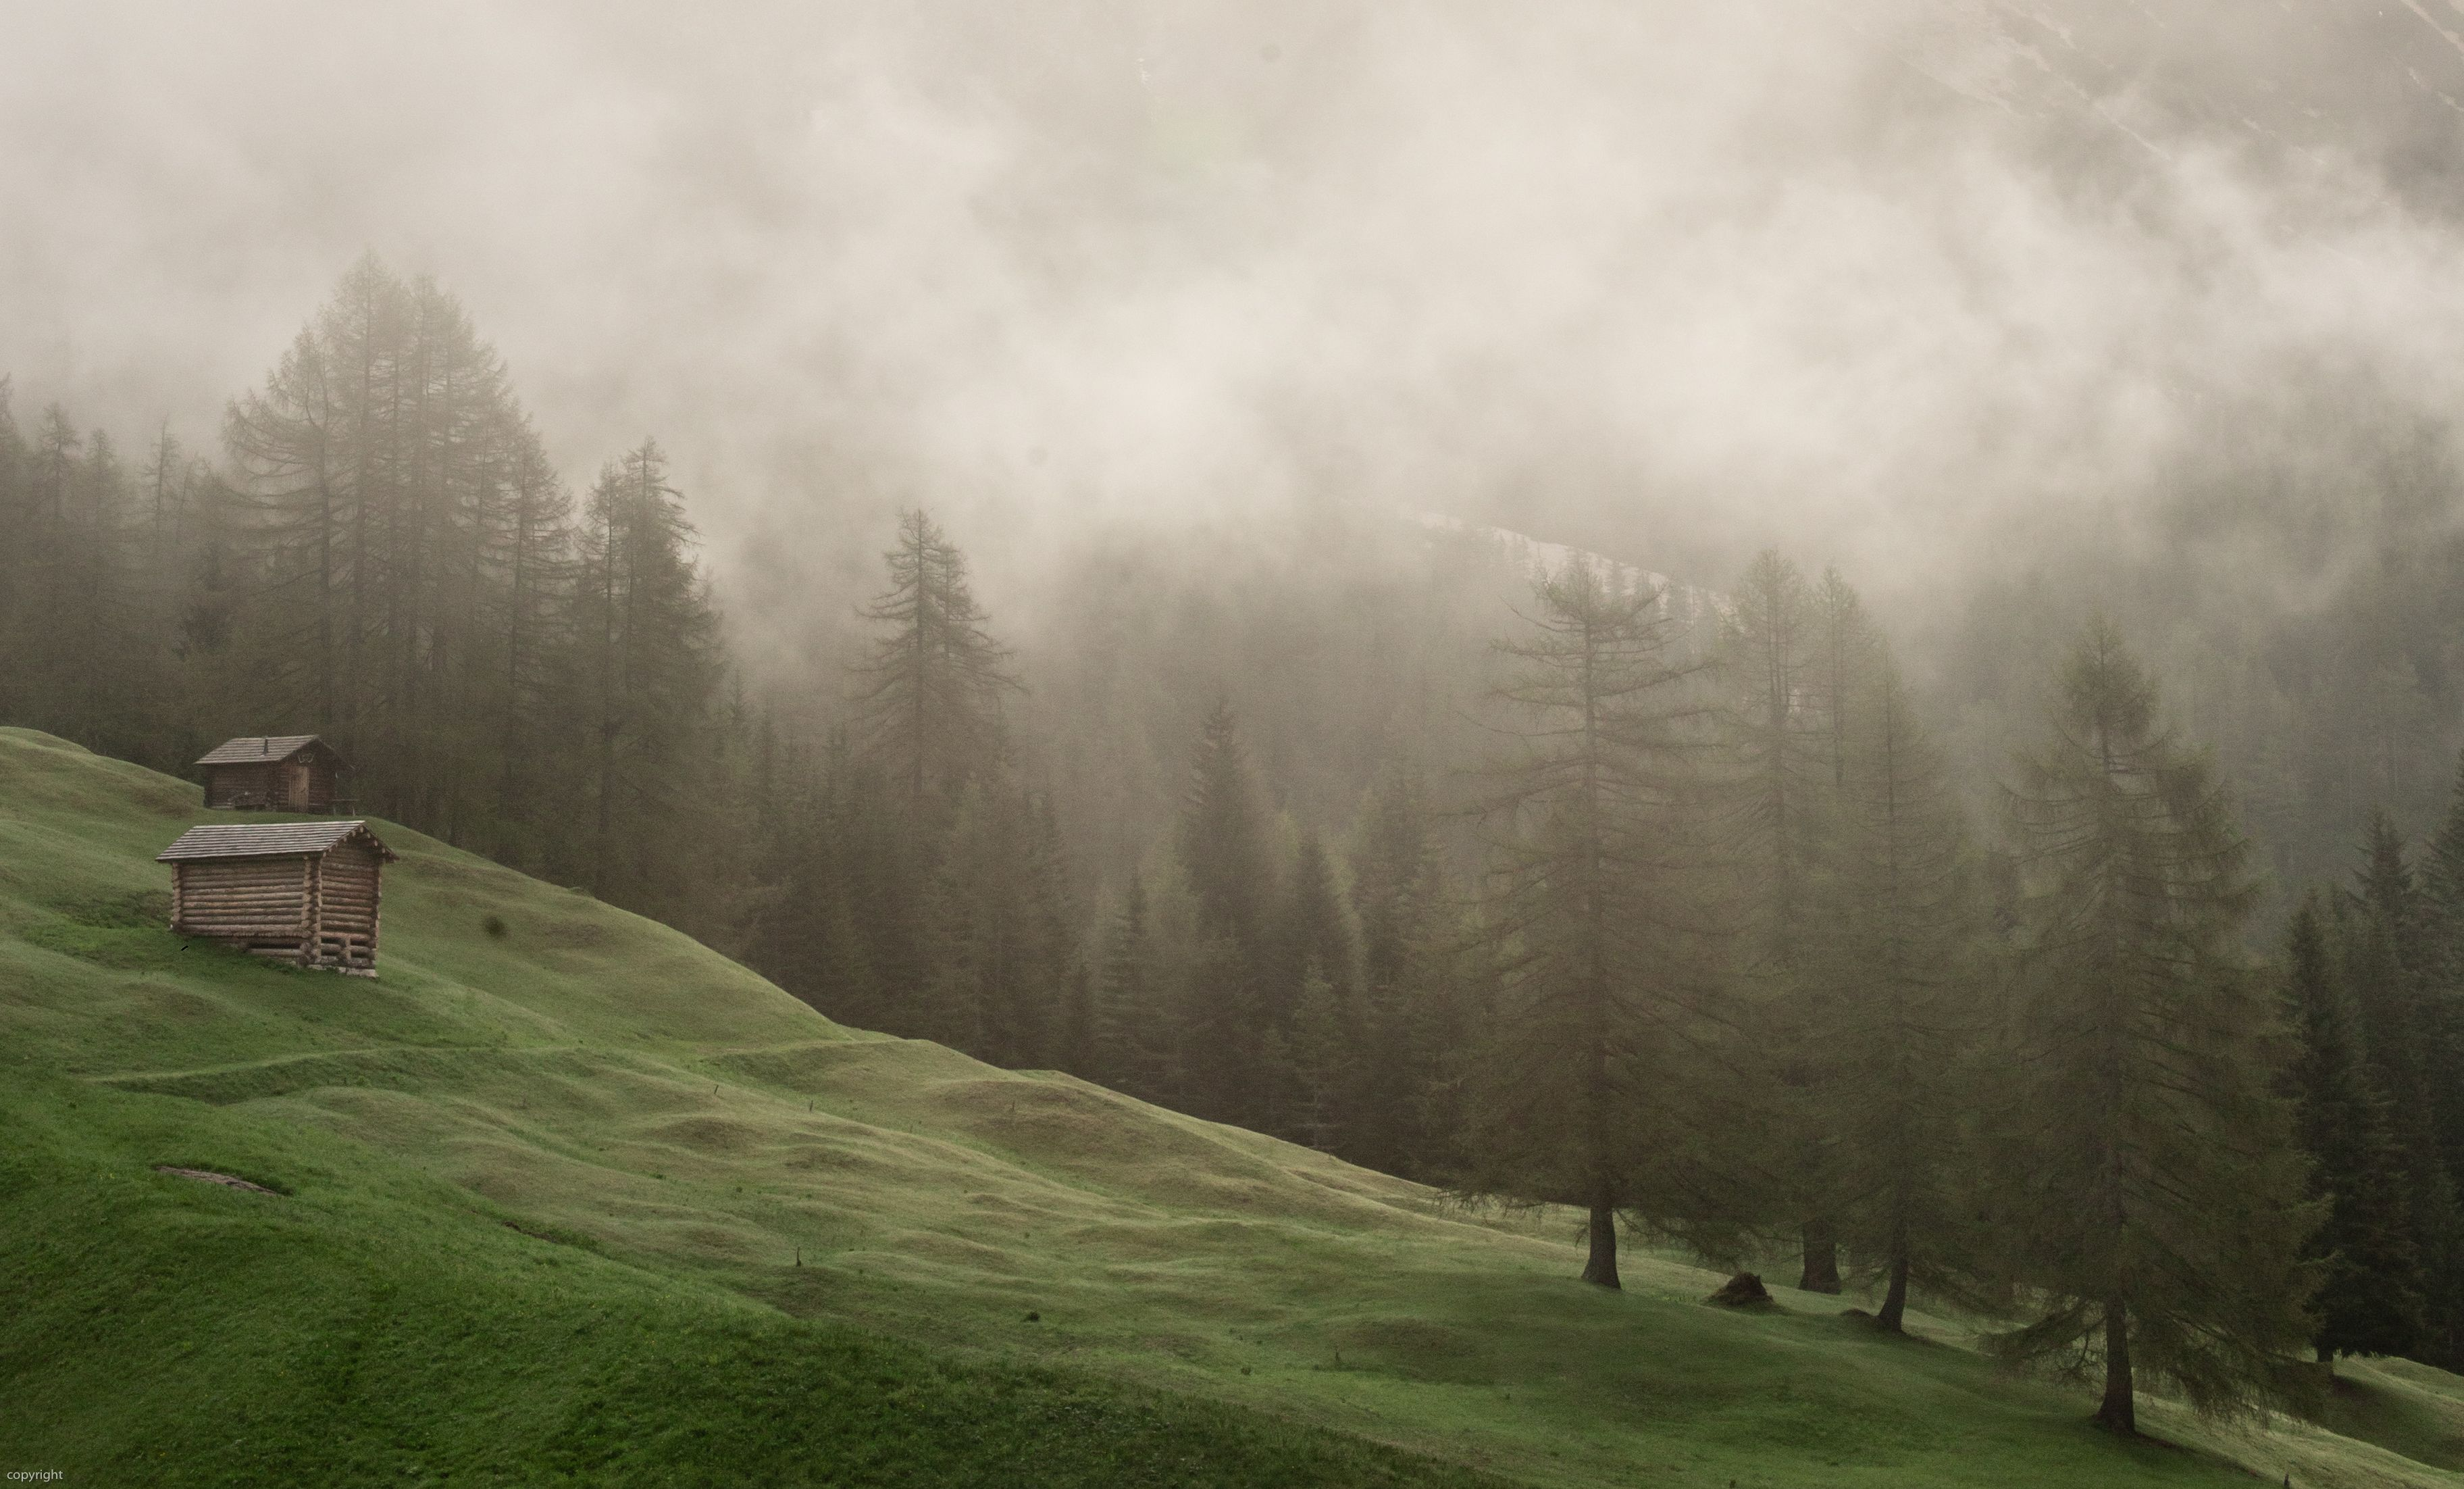
\includegraphics[width=0.8\linewidth]{images/1.jpg}
    \caption{Hehe}
    \label{fig:tintin}
\end{figure}

\vspace{0.5cm}

hello this is saklain writing gibberish.

In FIgure~\ref{fig:tintin}, we see that we can go to this place and kill someone and hide the body easily.

\lipsum[1-2]

\begin{figure}[!ht]
    \centering
    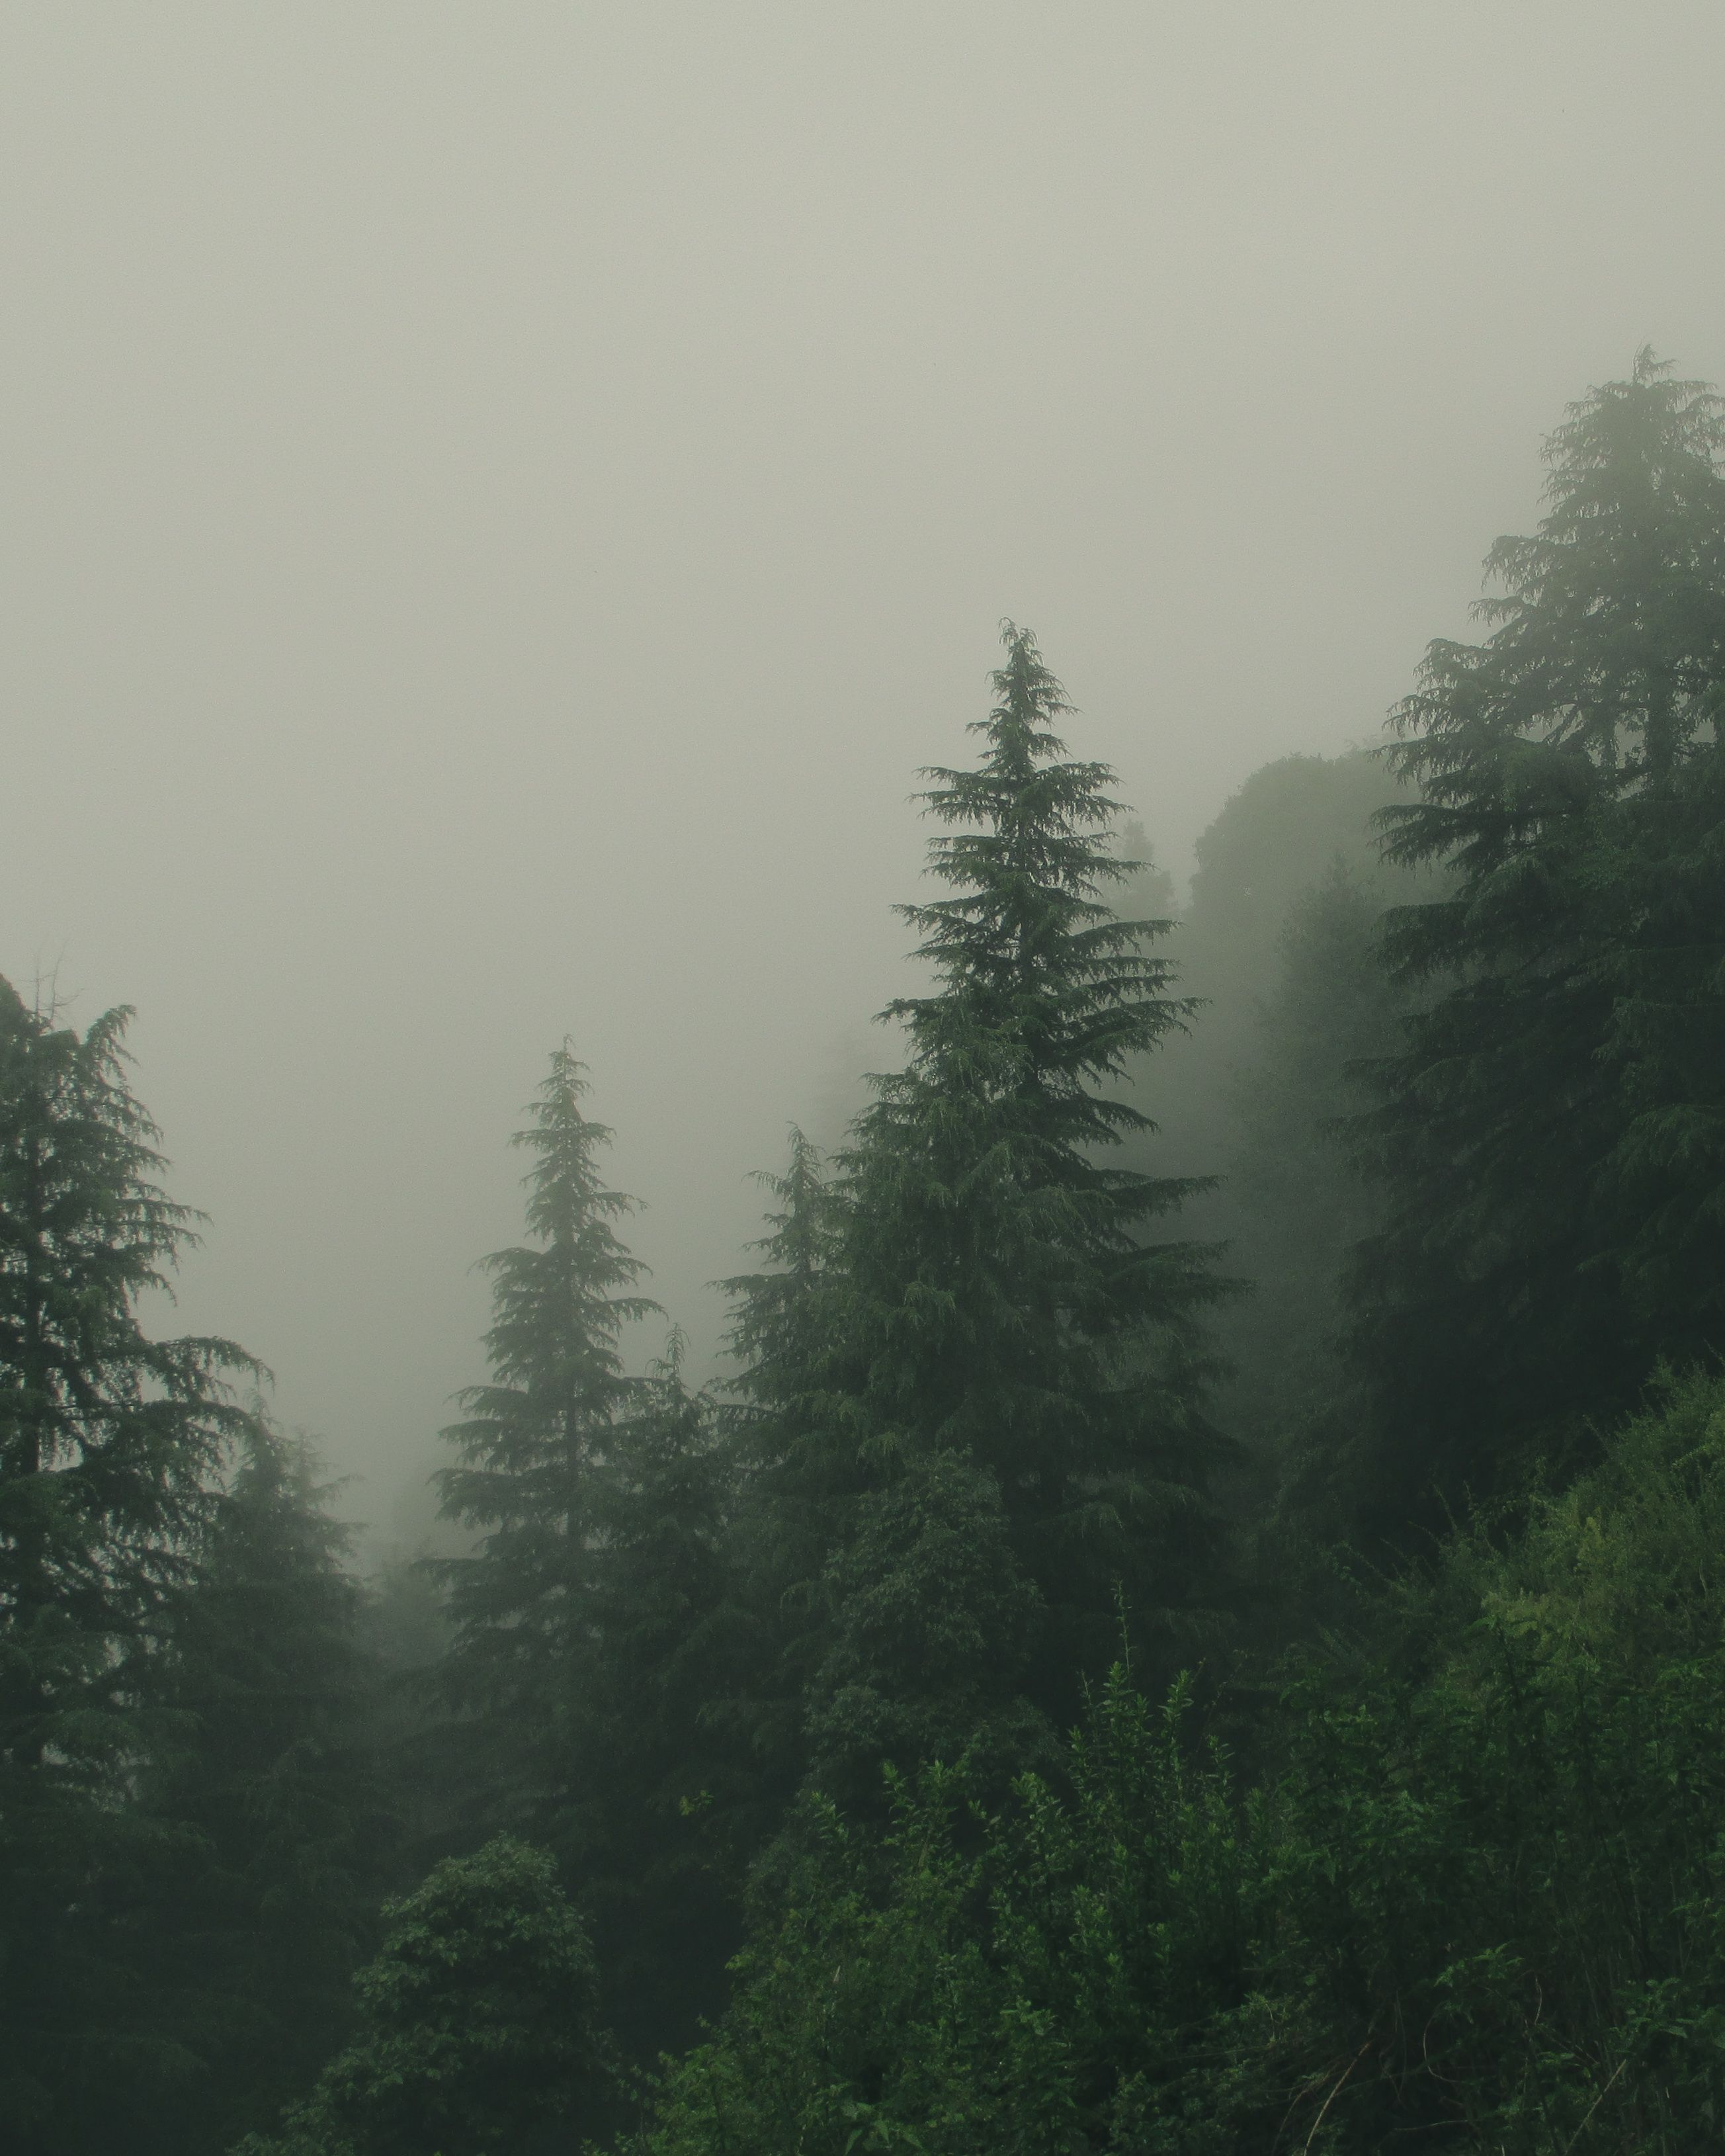
\includegraphics[width=0.8\linewidth]{images/2.jpg}
    \caption{Hehe}
    \label{fig:tintin1}
\end{figure}

\lipsum[1-2]

\begin{figure}[!ht]
    \centering
    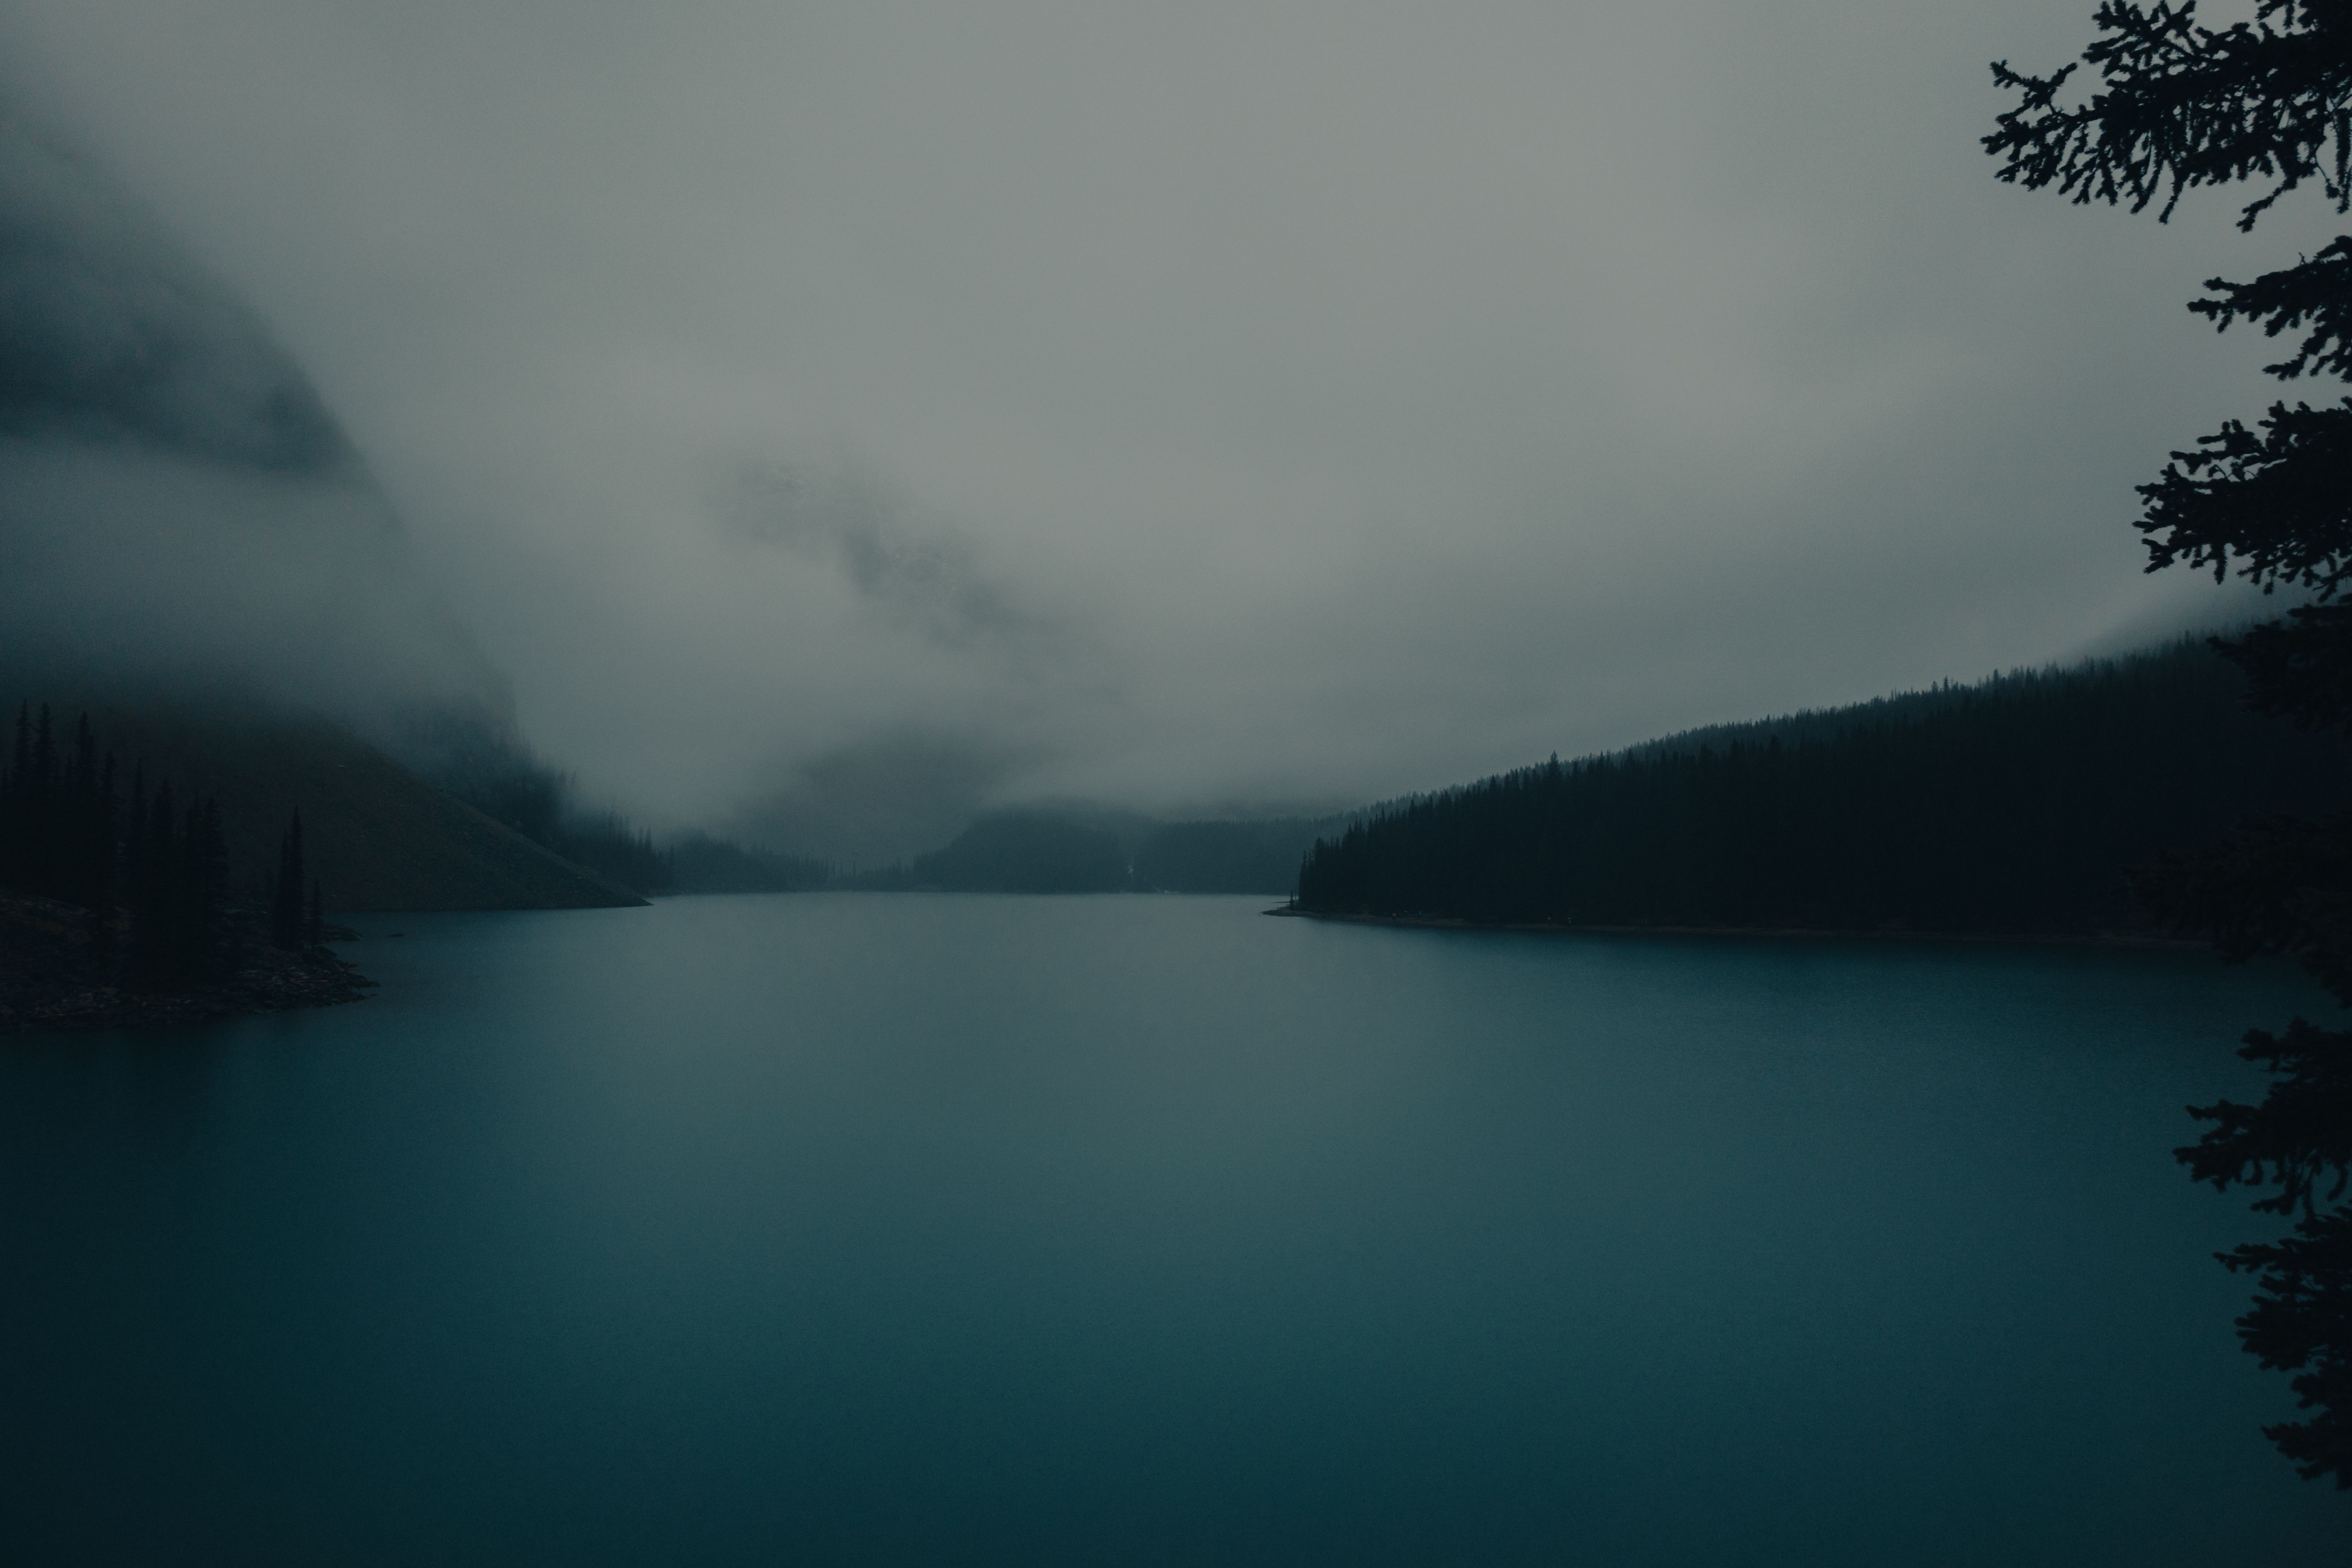
\includegraphics[width=0.8\linewidth]{images/3.jpg}
    \caption{Hehe}
    \label{fig:tintin2}
\end{figure}

\begin{figure}[!ht]
    \centering
    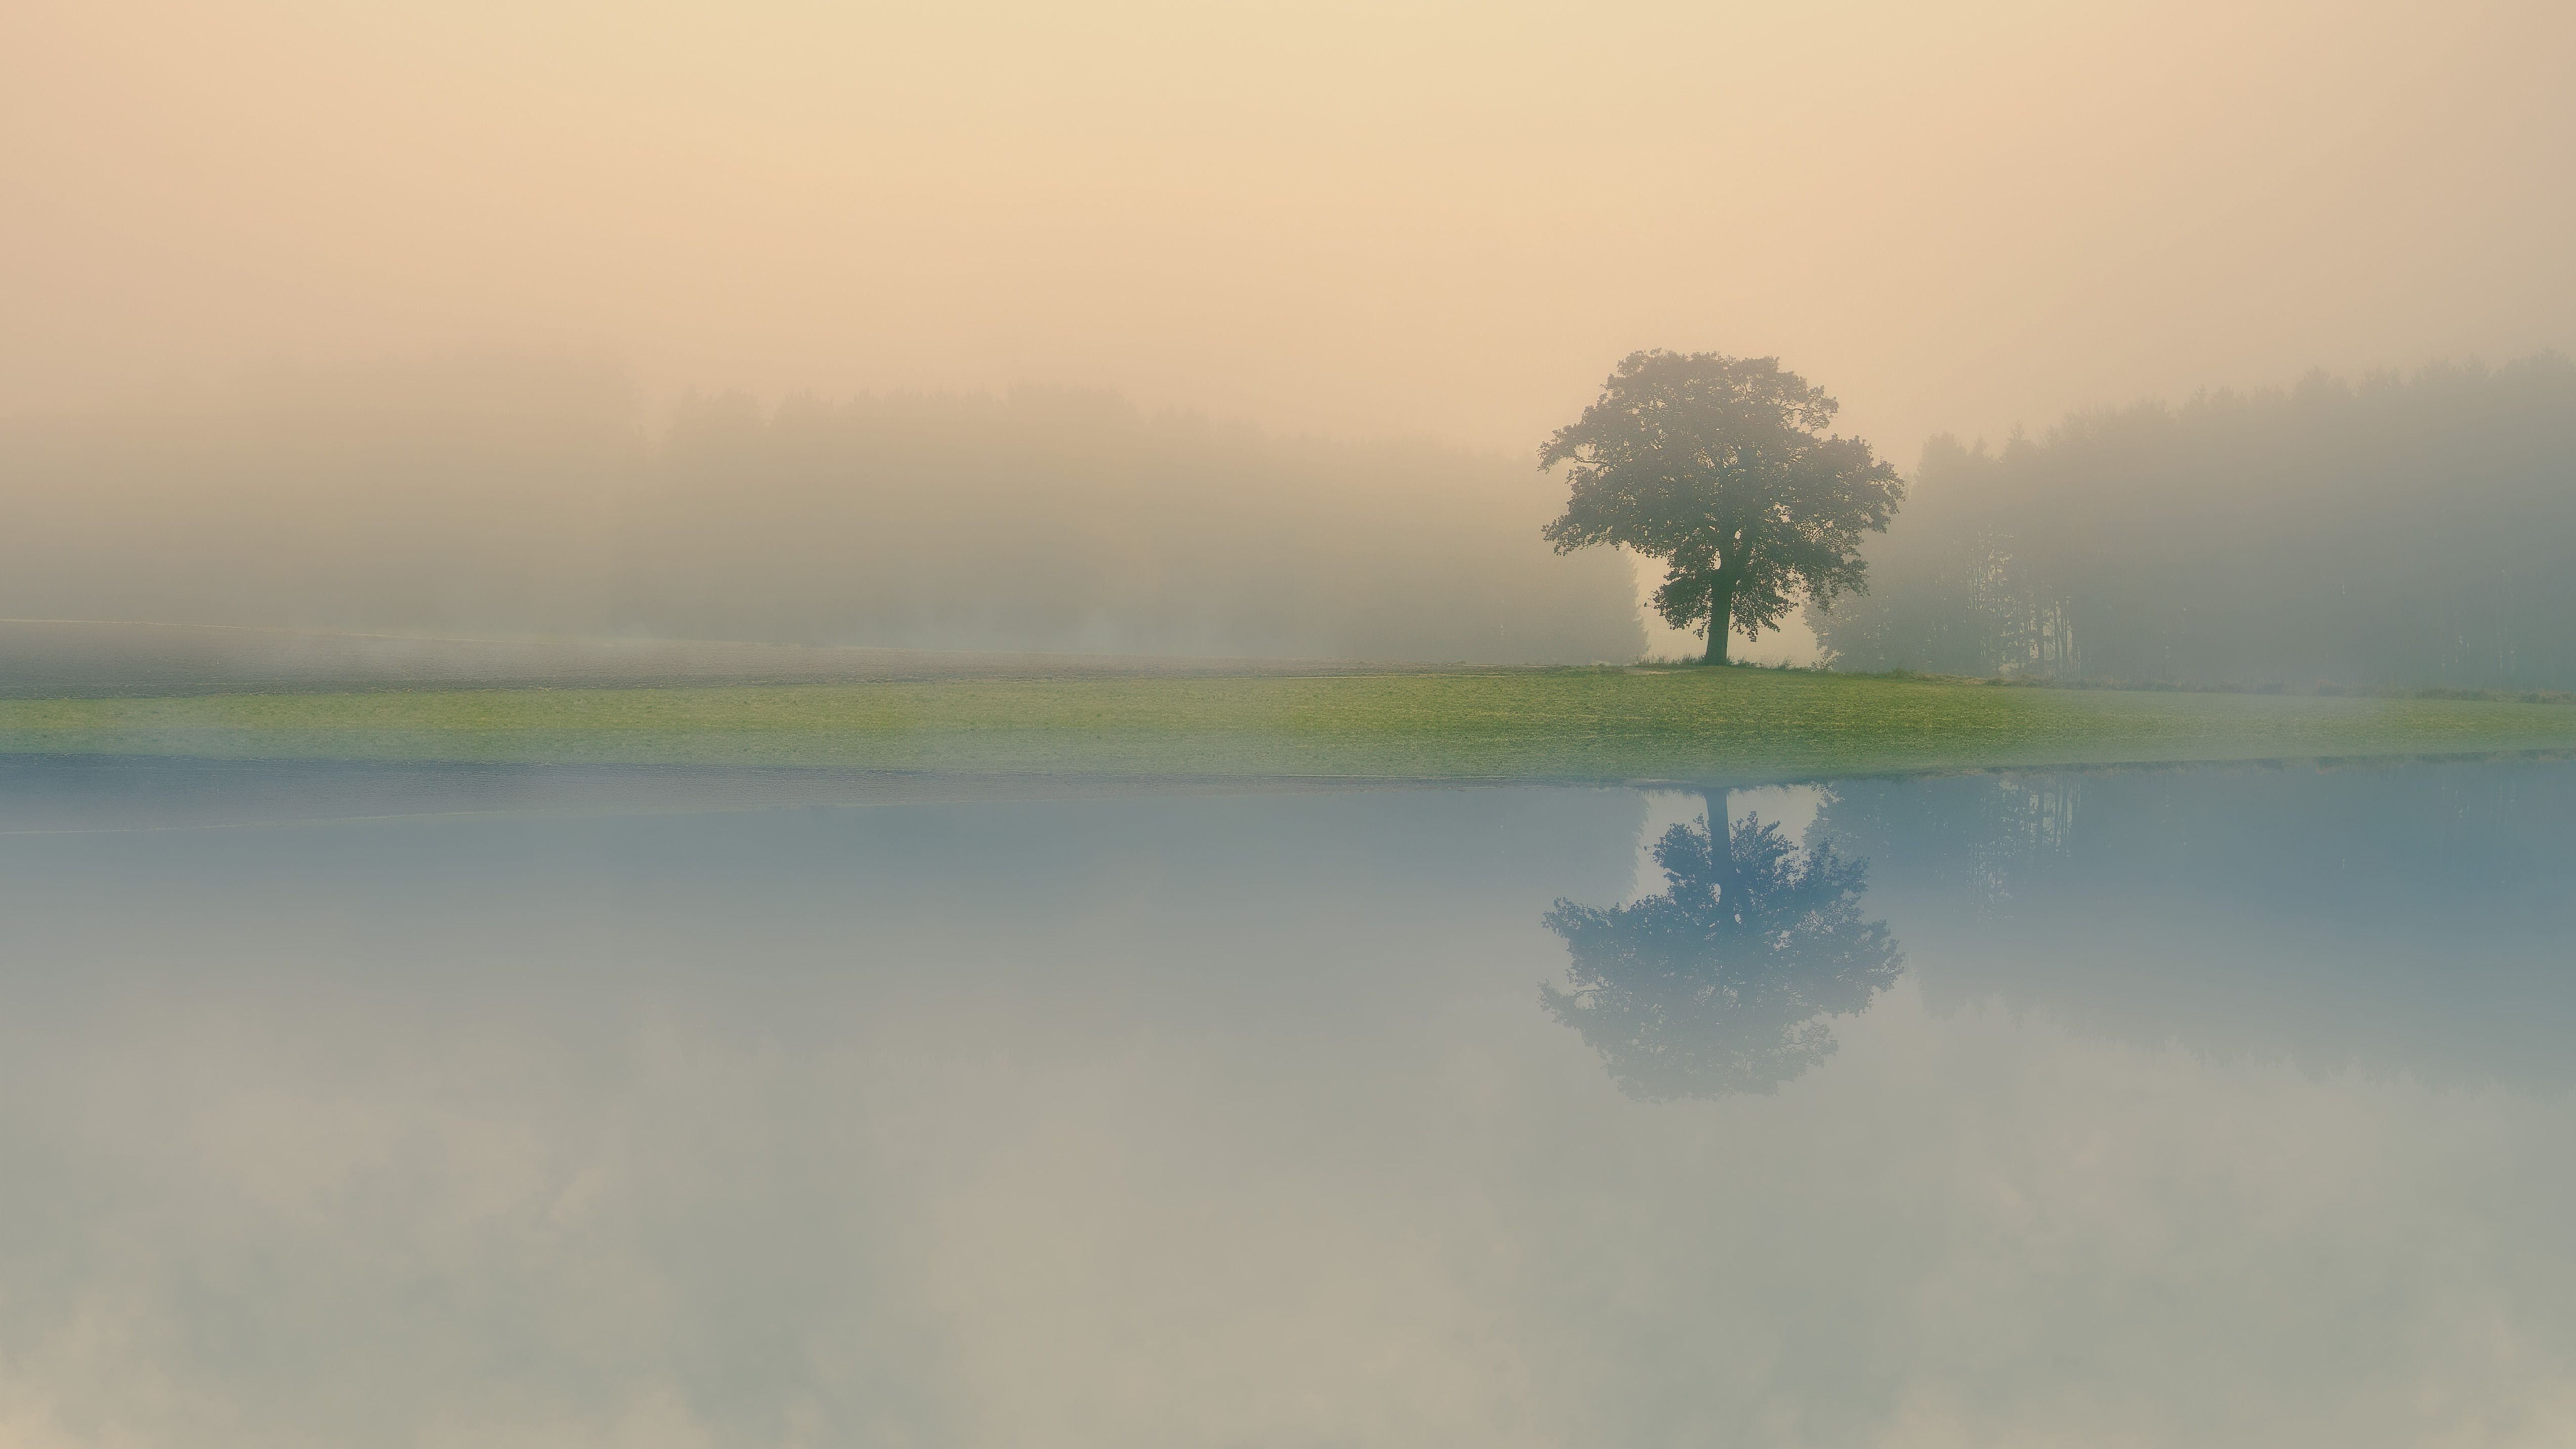
\includegraphics[width=0.8\linewidth]{images/4.jpg}
    \caption{Hehe}
    \label{fig:tintin3}
\end{figure}

\lipsum[1-2]

% \linewidth -> width of line.... double column niye likhle per line and \textwidth hocche total text er width.... borota


\begin{figure}[!htbp]
    \centering
    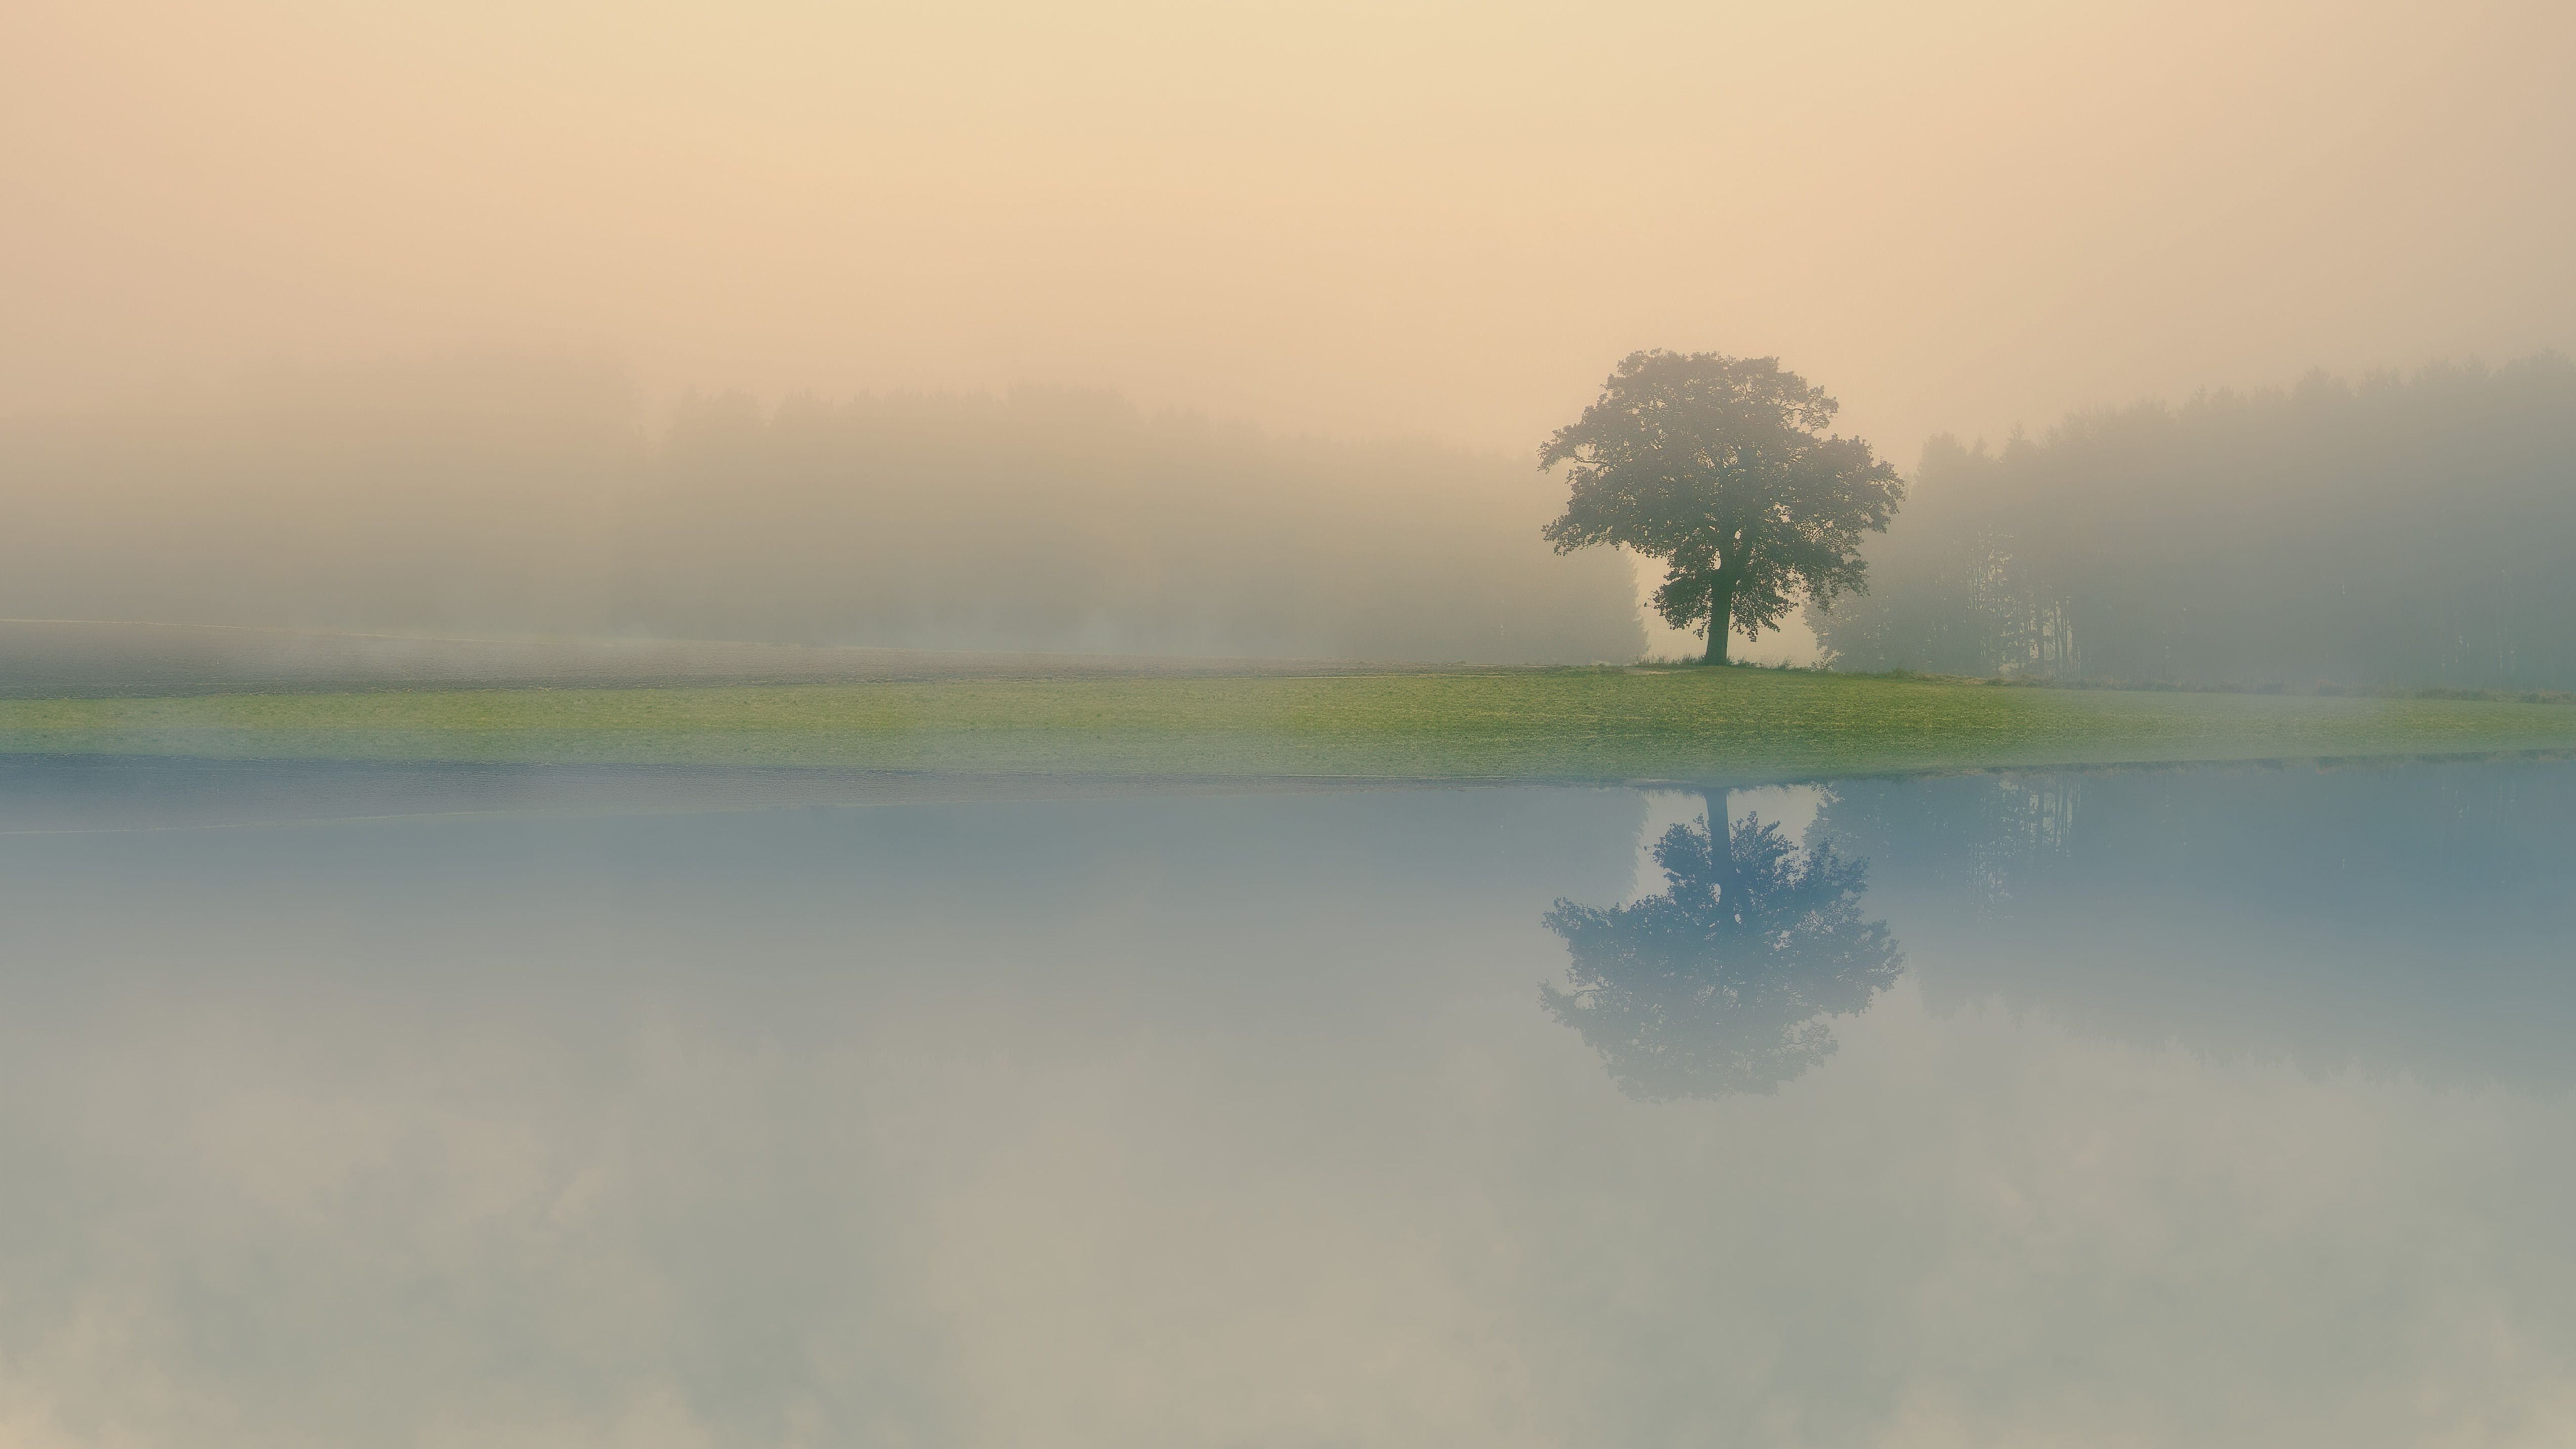
\includegraphics[width=0.8\linewidth]{images/4.jpg}
    \caption{Hehe}
    \label{fig:tintin4}
\end{figure}


\begin{figure}[!htbp]
    \centering
    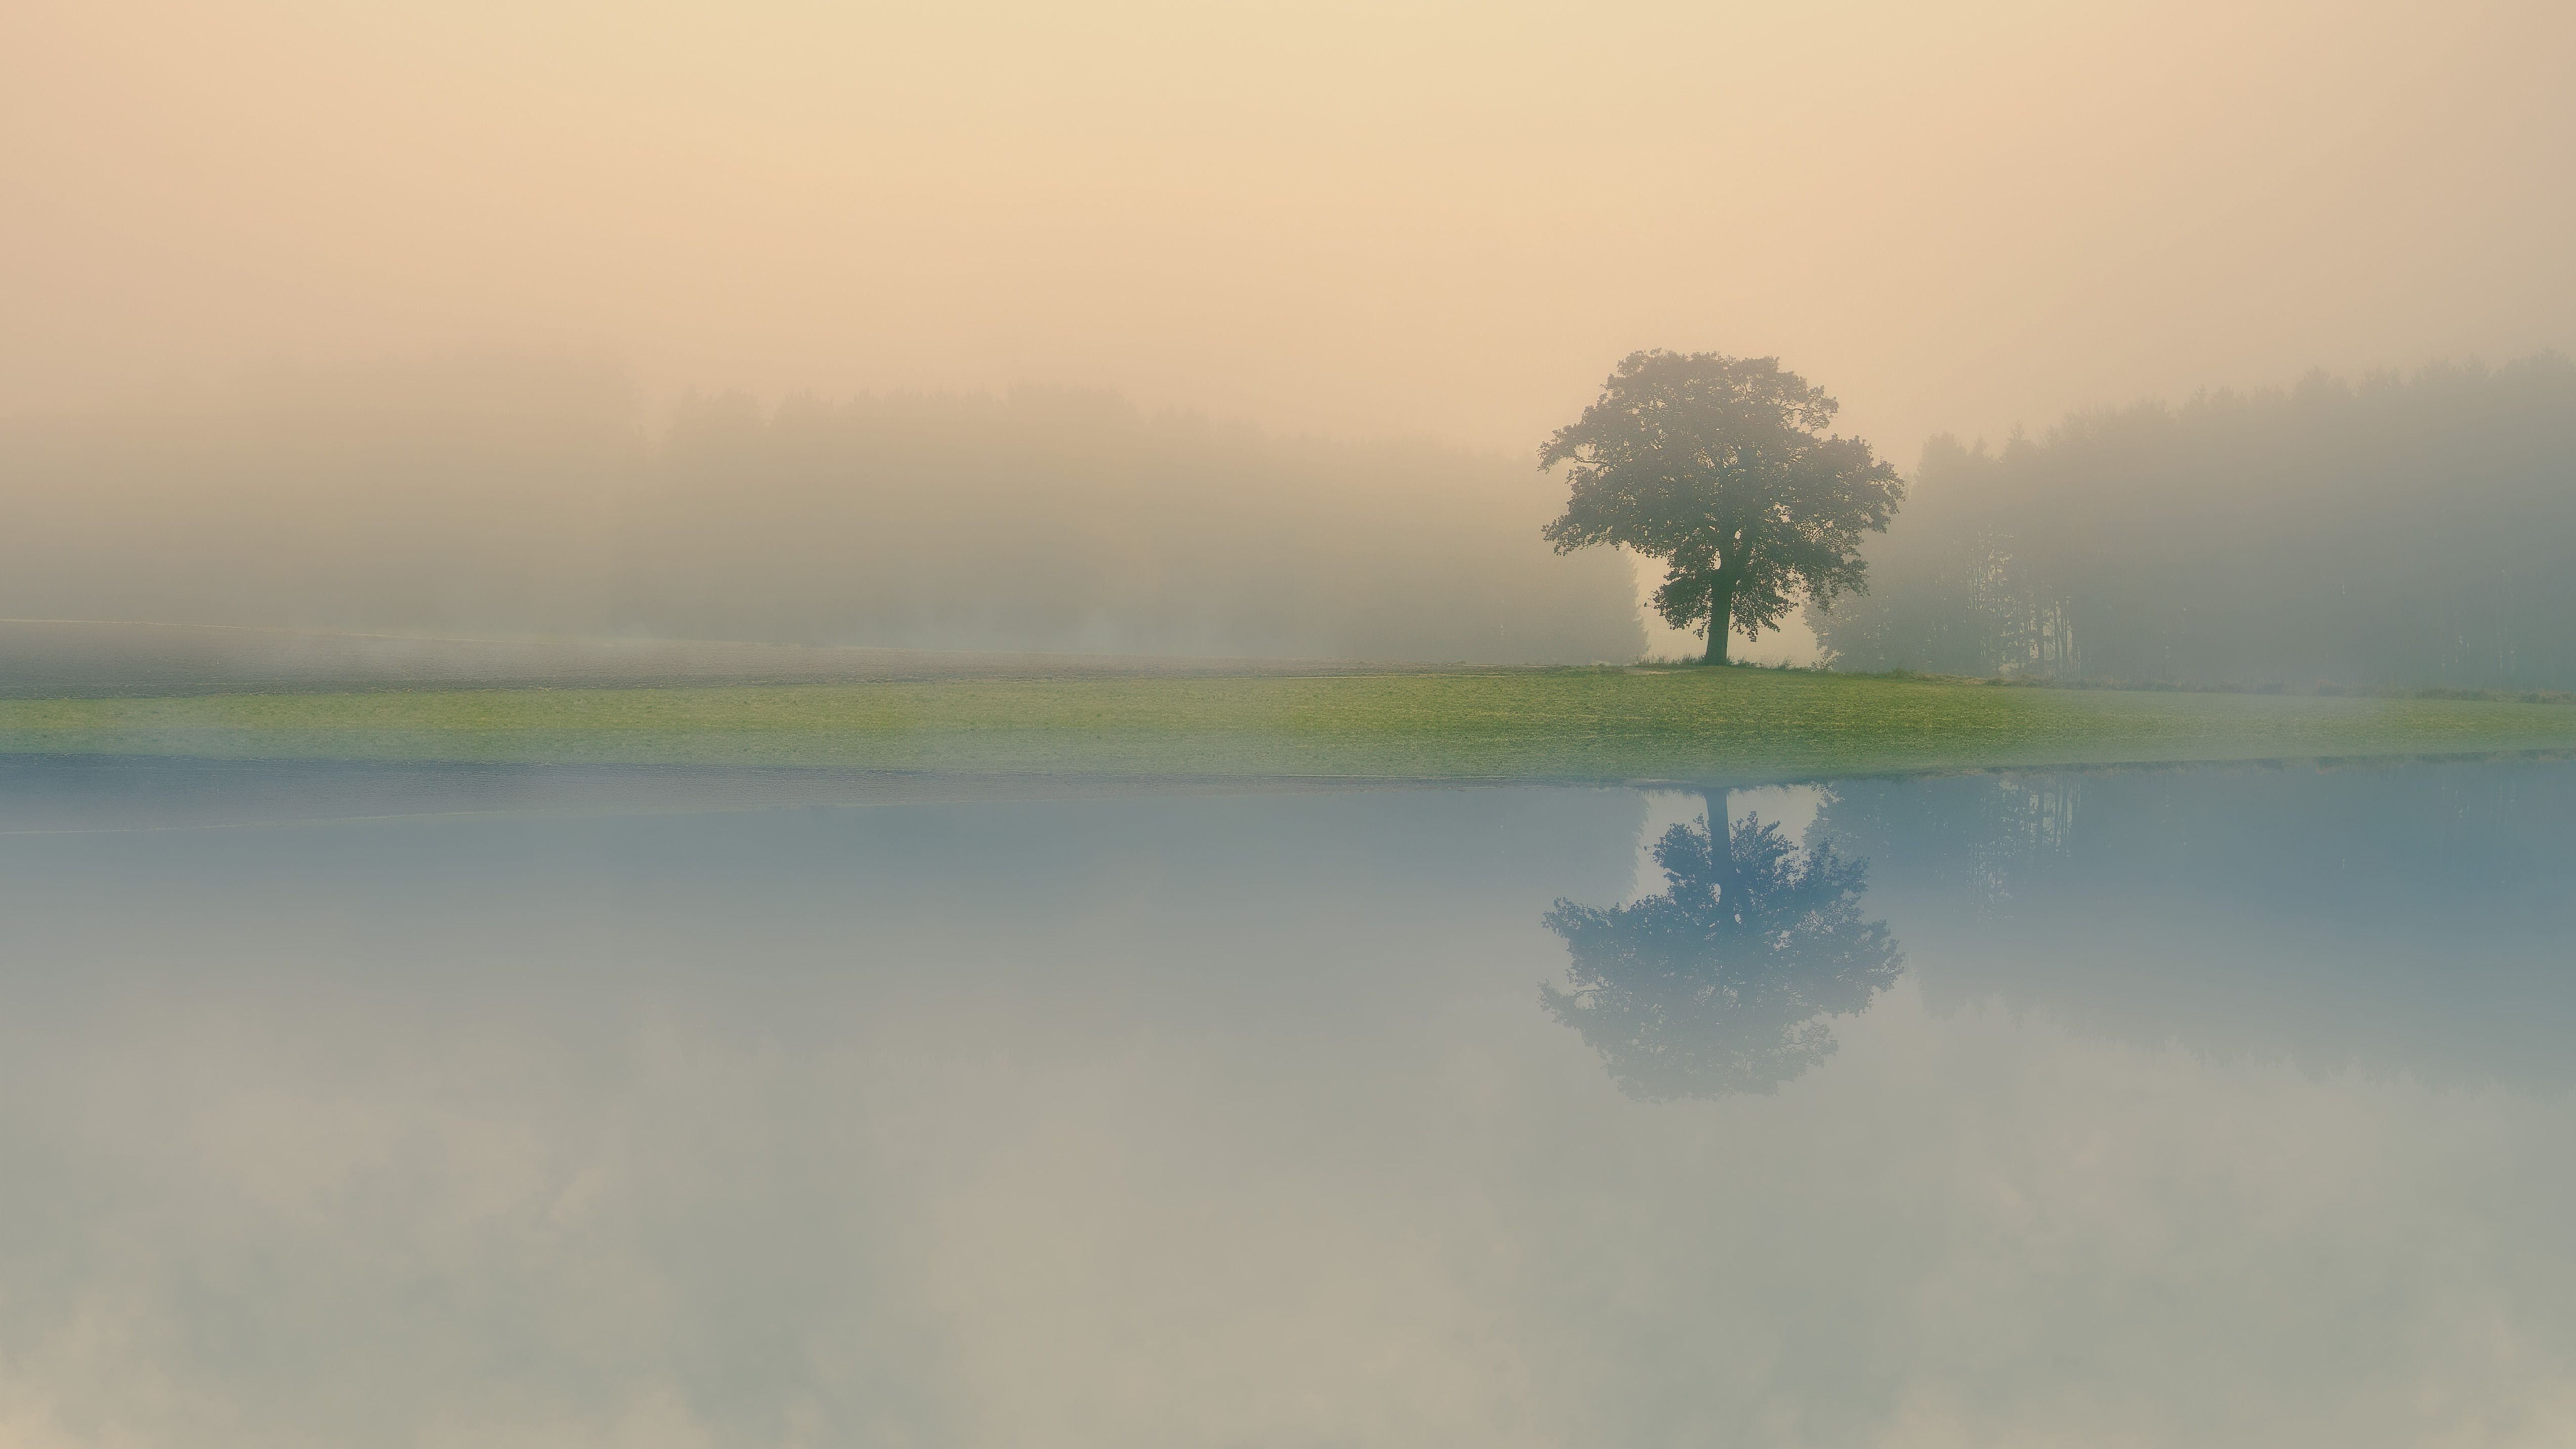
\includegraphics[scale=.026]{images/4.jpg}  % sclae hocche real image er koto percent size nibe
    \caption{Hehe}
    \label{fig:tintin5}
\end{figure}


\begin{figure}[!htbp]
    \centering
    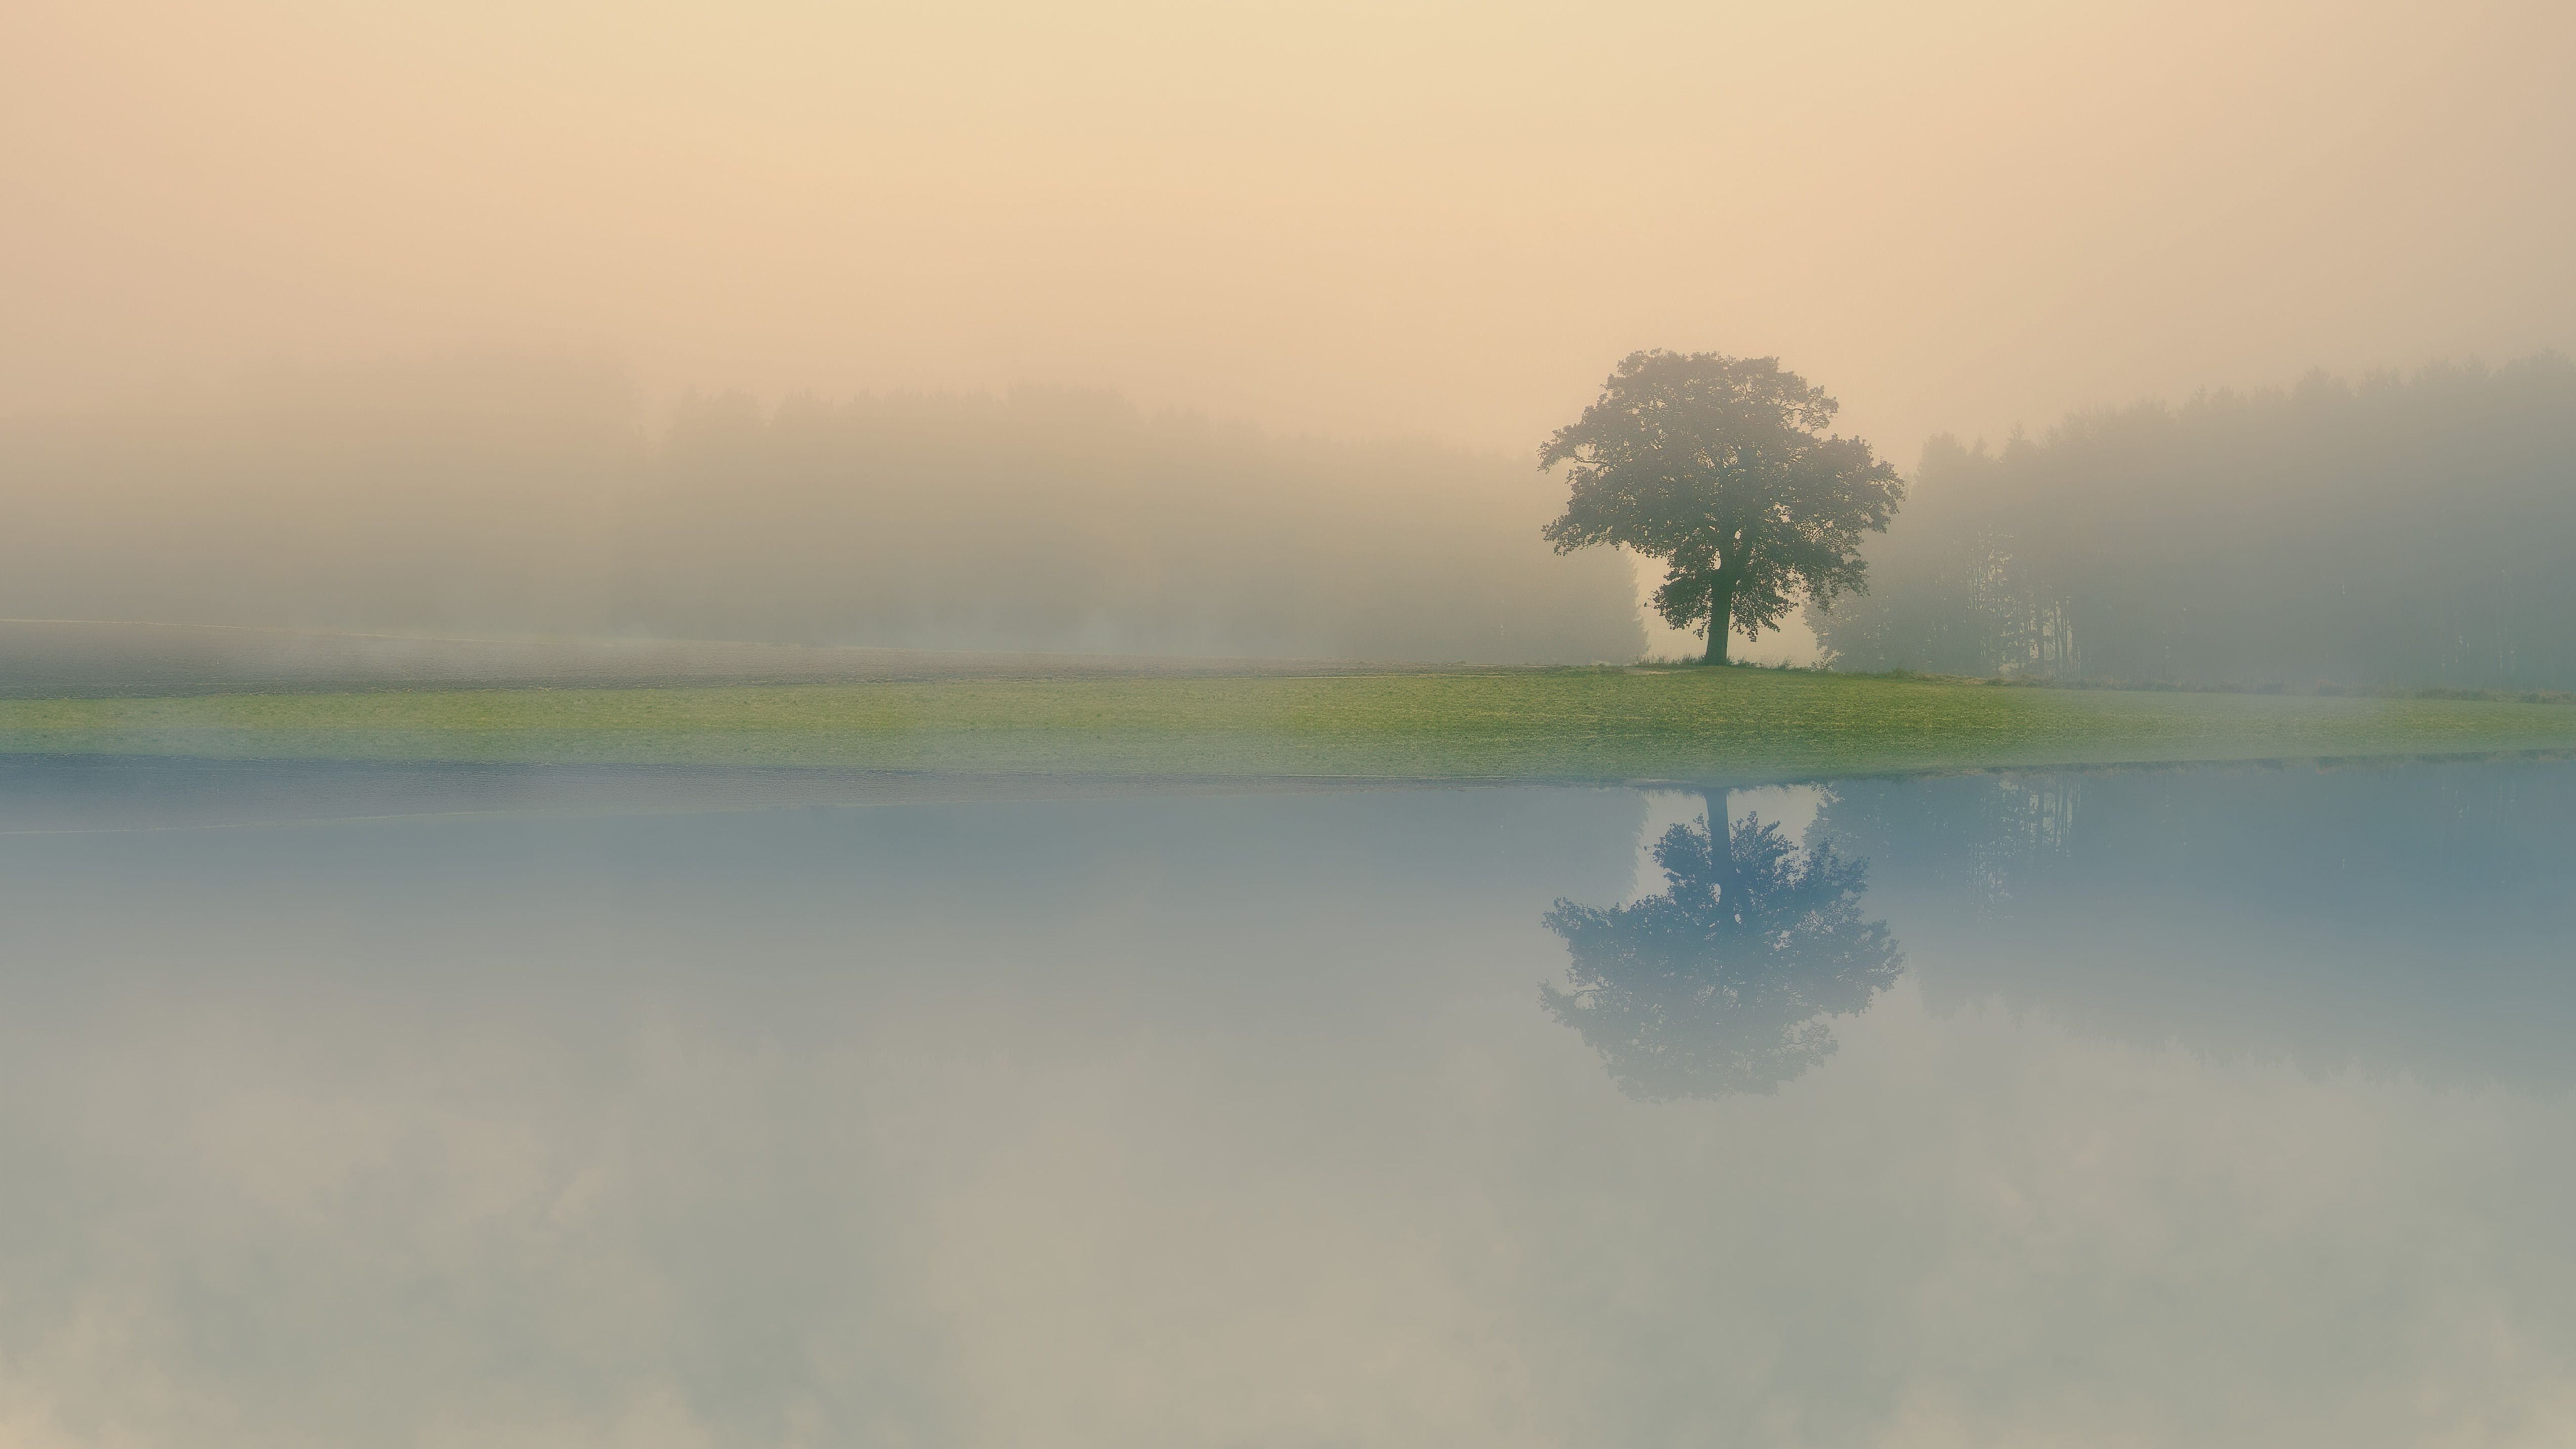
\includegraphics[width=0.4\linewidth, angle=5.9]{images/4.jpg}
    \caption{Hehe}
    \label{fig:tintin6}
\end{figure}

\vspace{1cm}

\subsection{Wrapped figure}

\lipsum[1-2]
\begin{wrapfigure}{r}{0.6\linewidth}
    \centering
    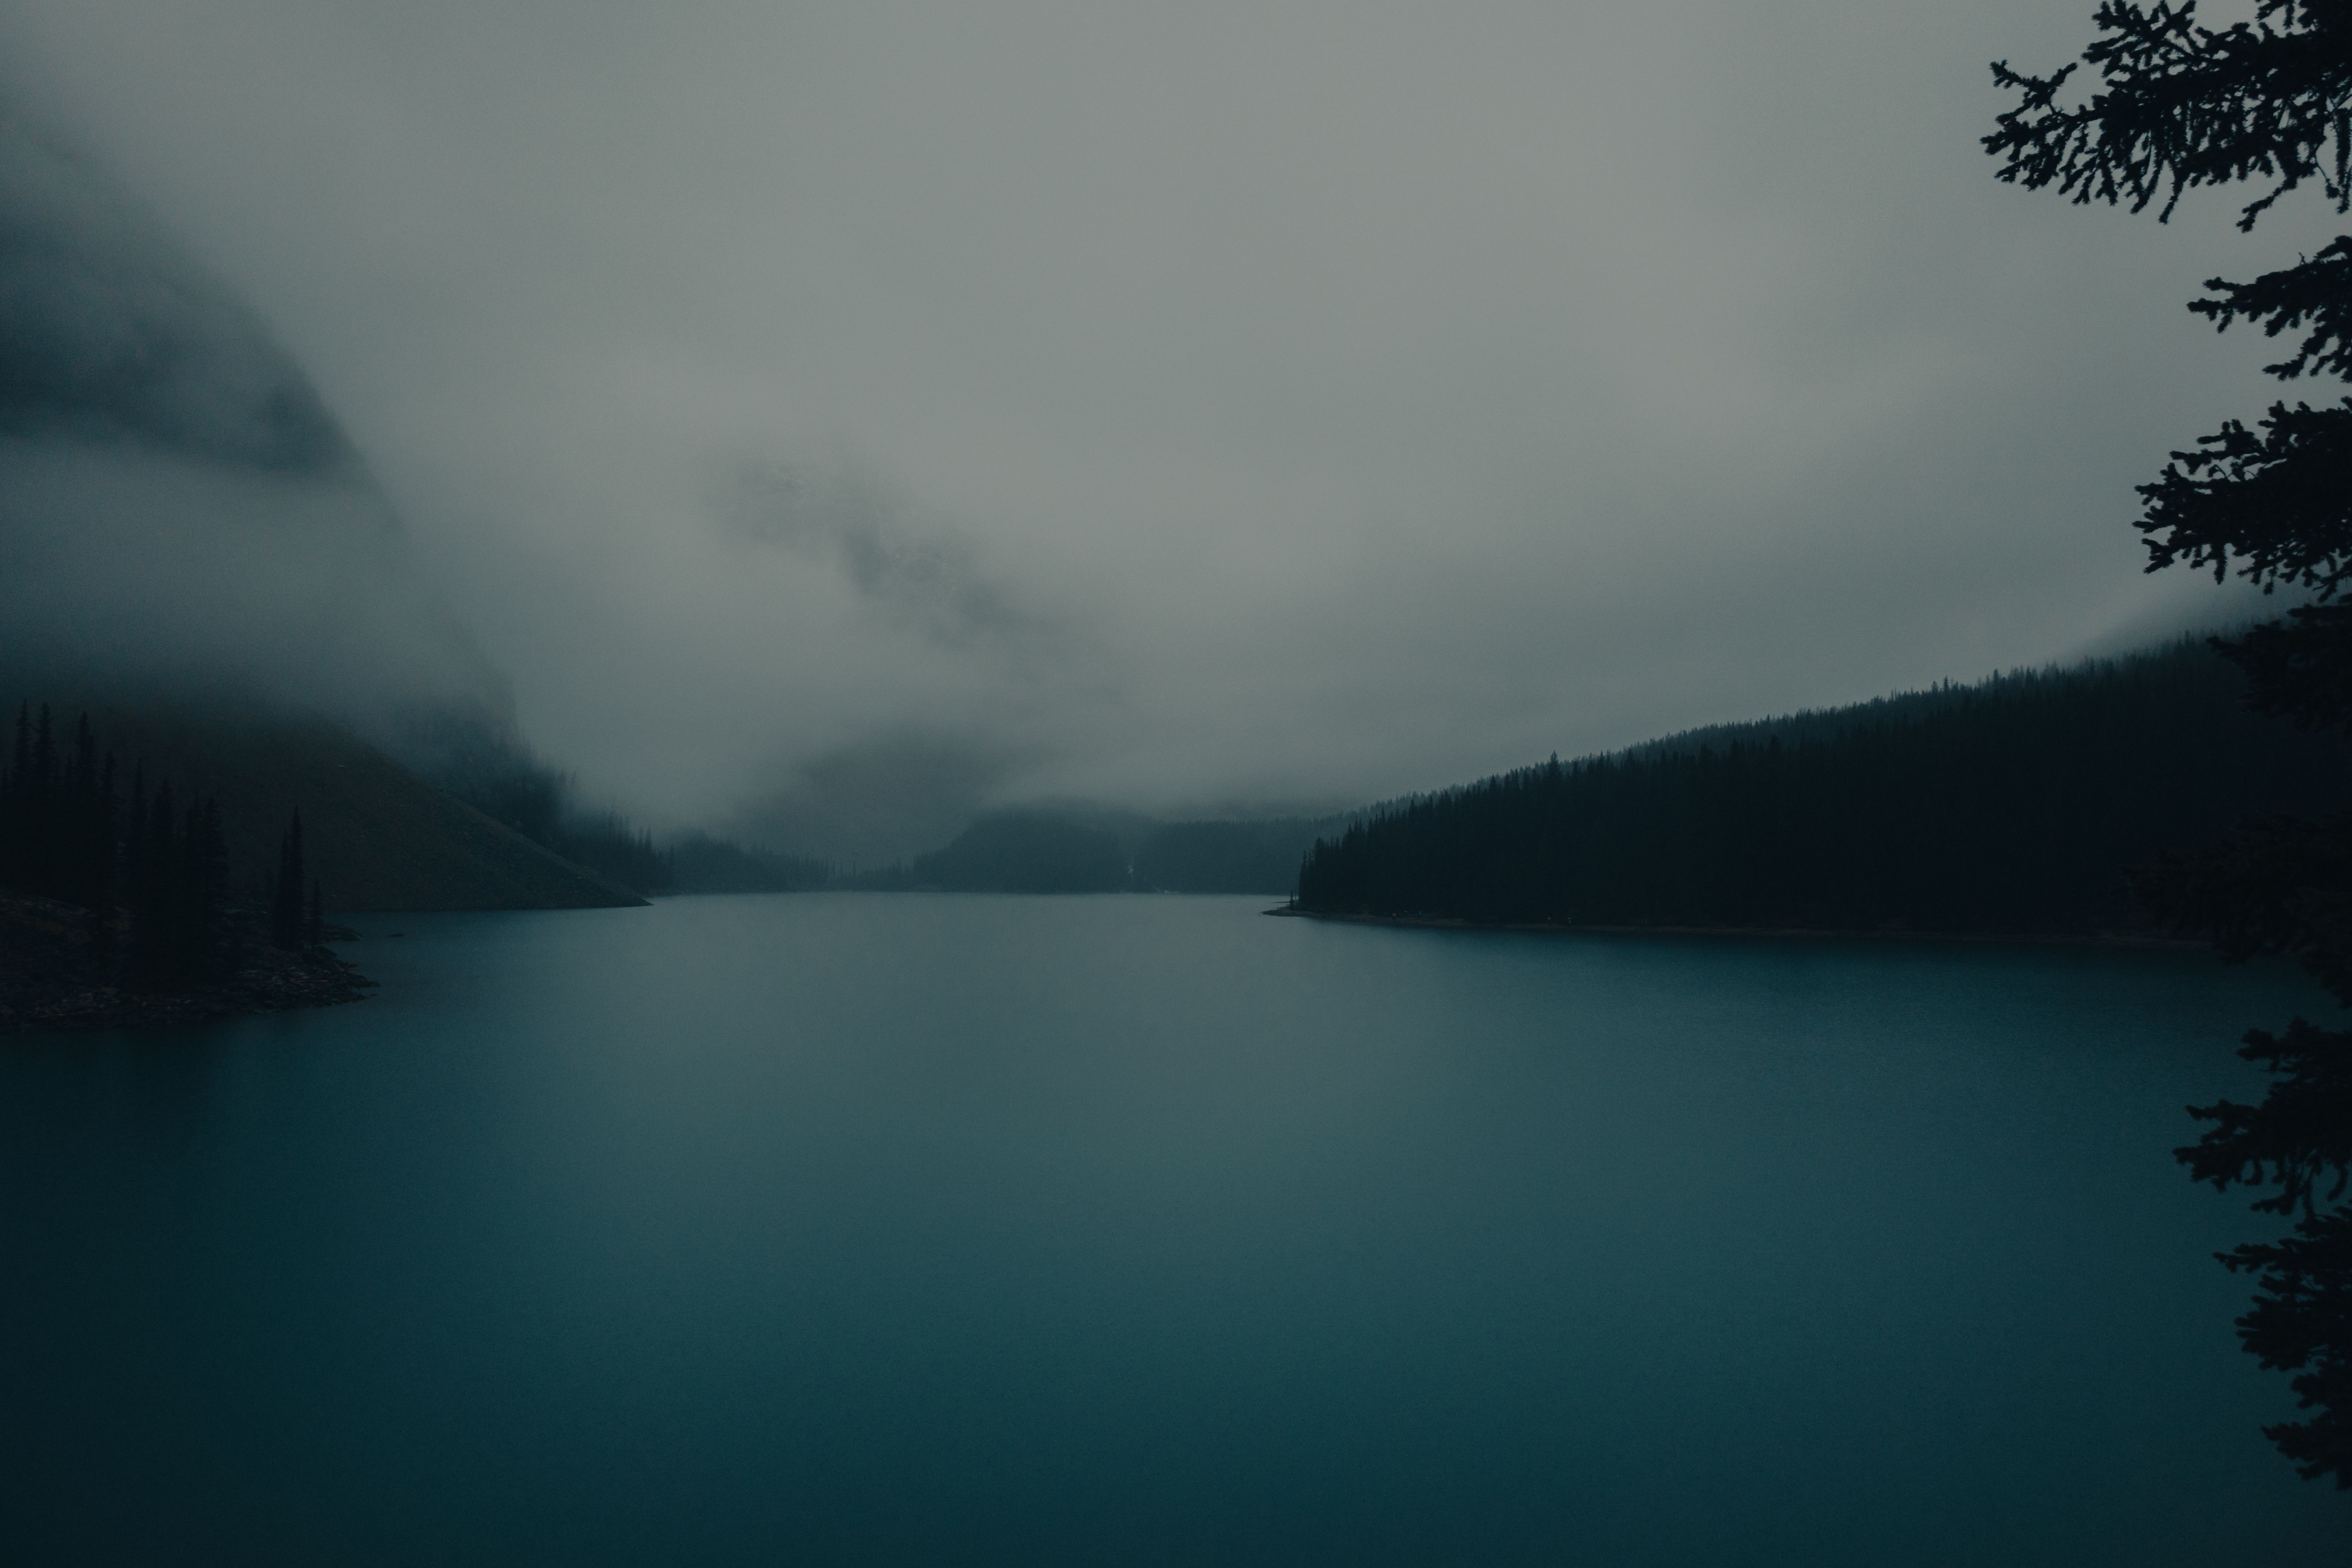
\includegraphics[width=0.7\linewidth]{images/3.jpg}
    \caption{Saklain is dead}
    \label{fig:death}
\end{wrapfigure}

\lipsum[2]


\subsection{Subfigures}

\begin{figure}[ht]
    \centering
    \begin{subfigure}{0.35\linewidth}
        \centering
        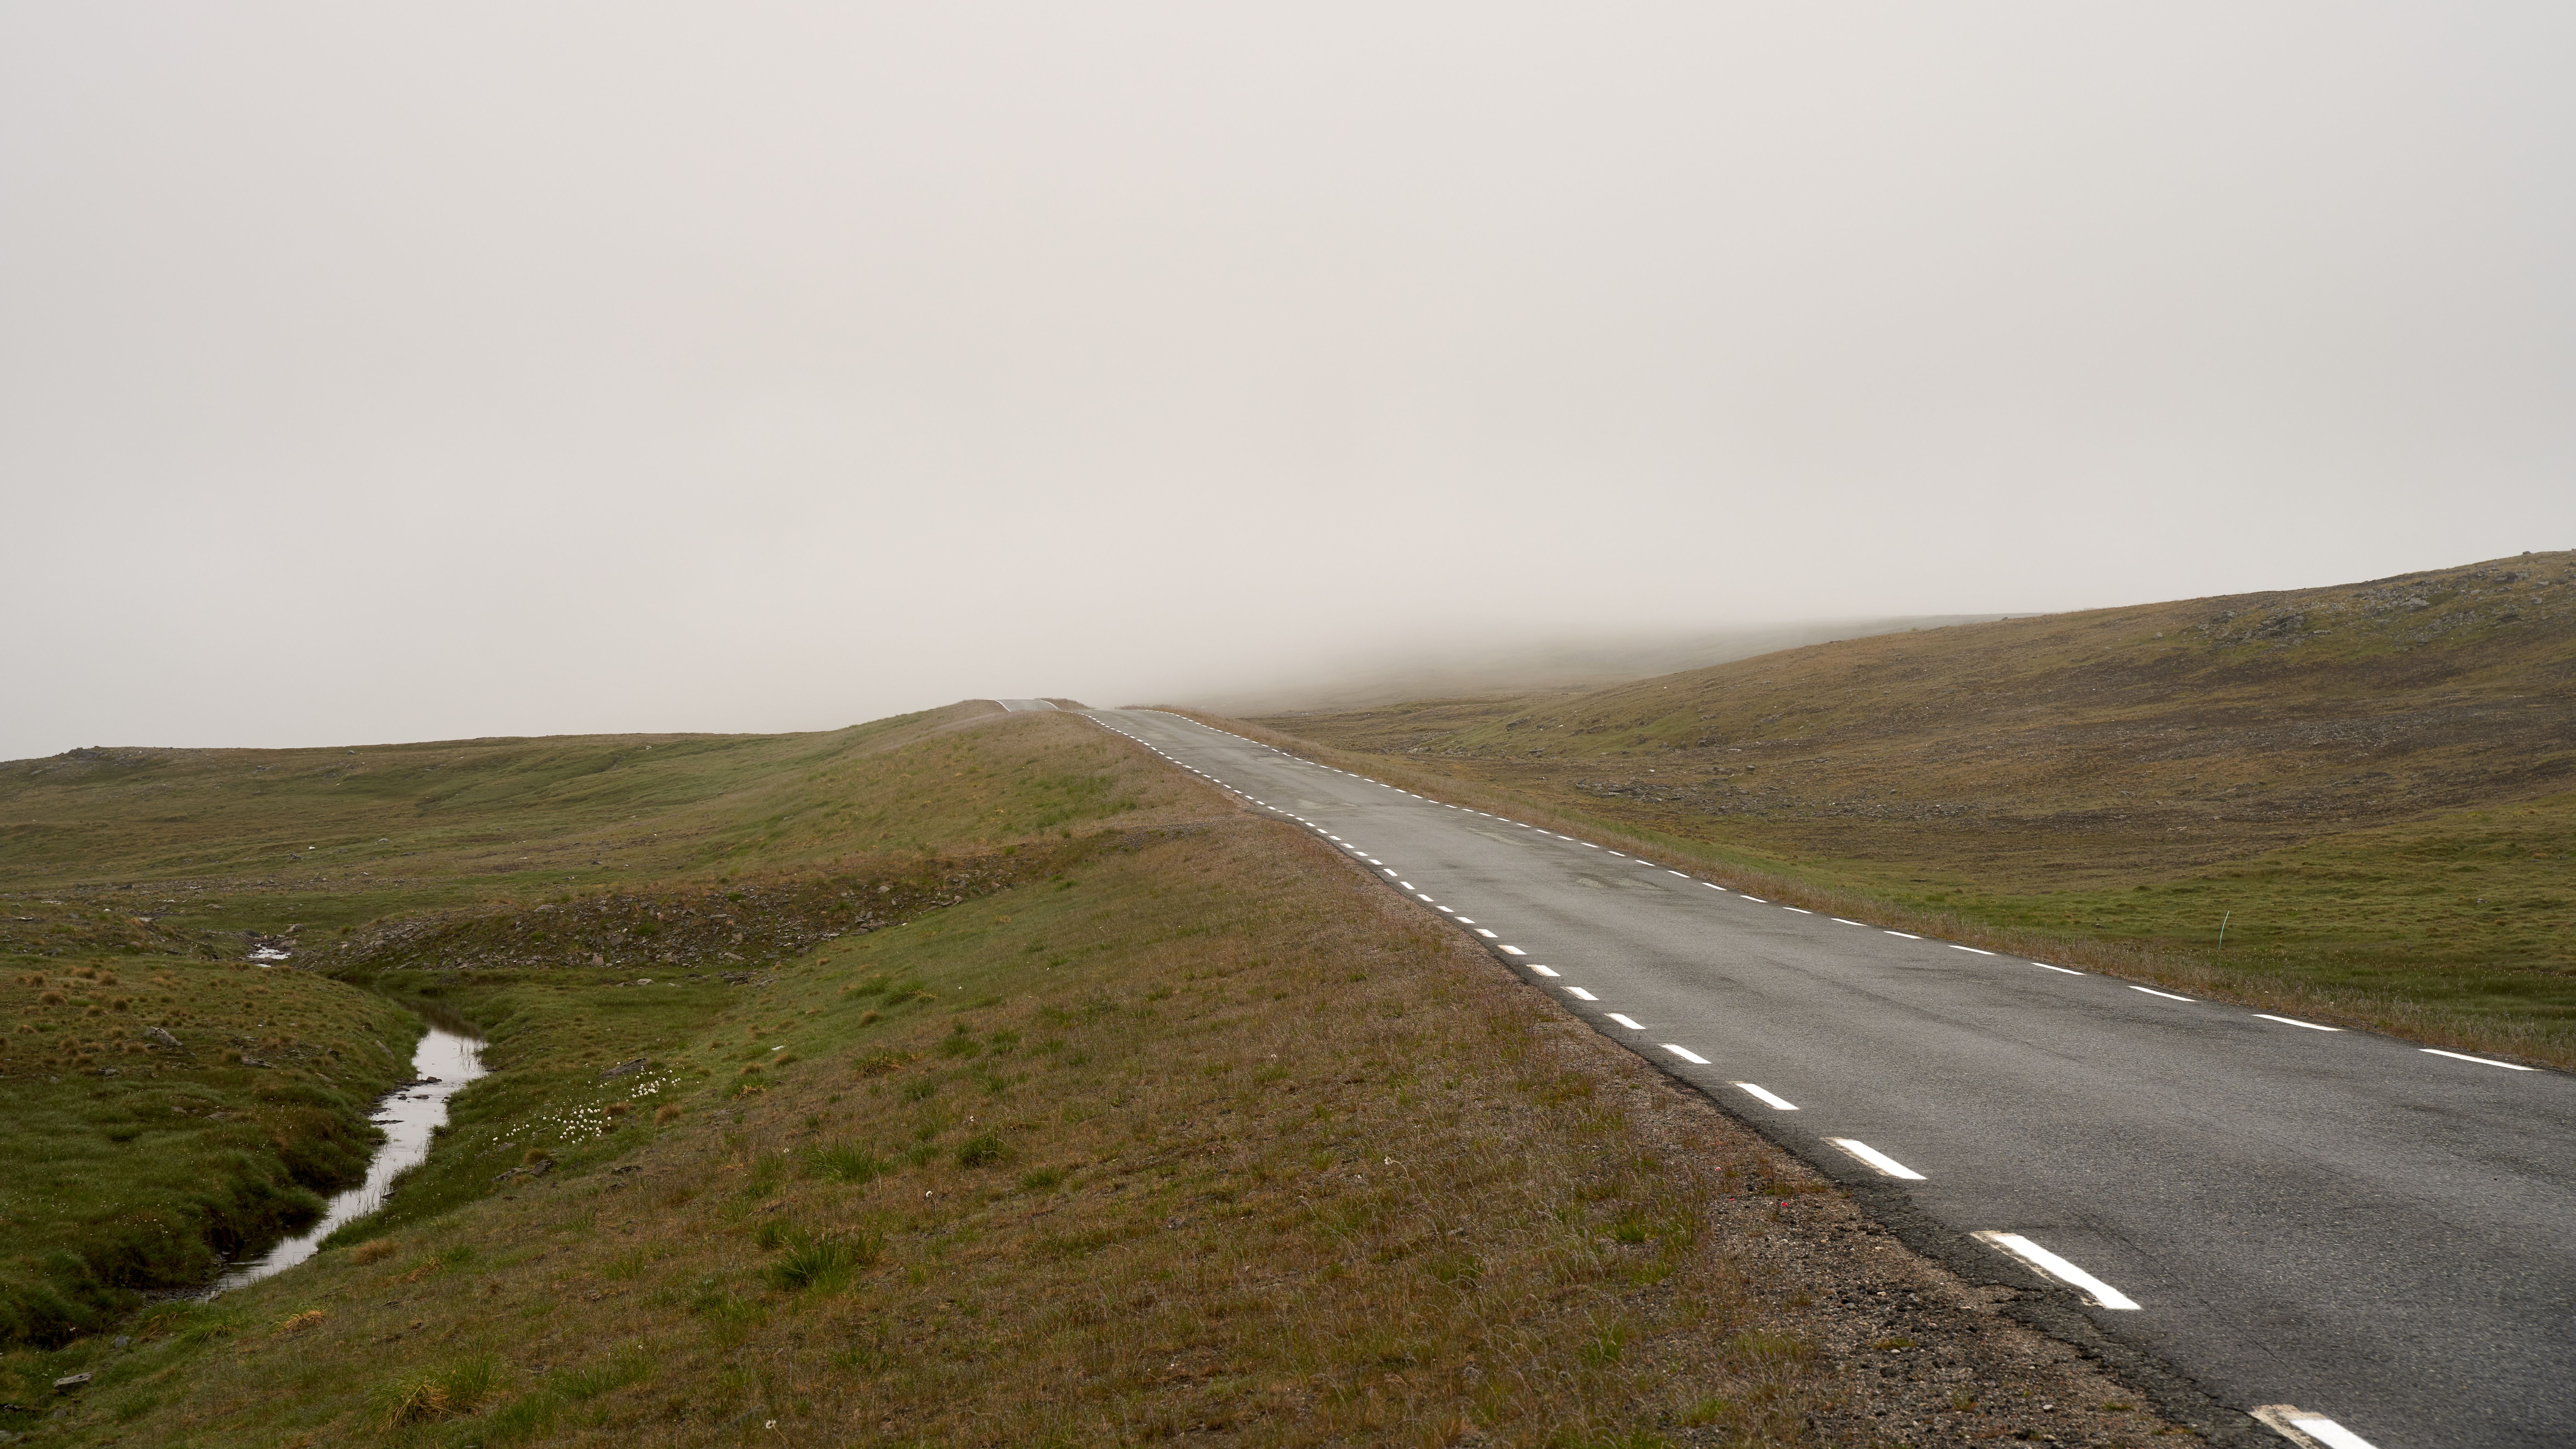
\includegraphics[width=.8\linewidth]{images/5.jpg}
        \caption{}
        \label{fig:life}
    \end{subfigure}
    \hfill % Adds horizontal stretching space between the two images
    \begin{subfigure}{0.35\linewidth}
        \centering
        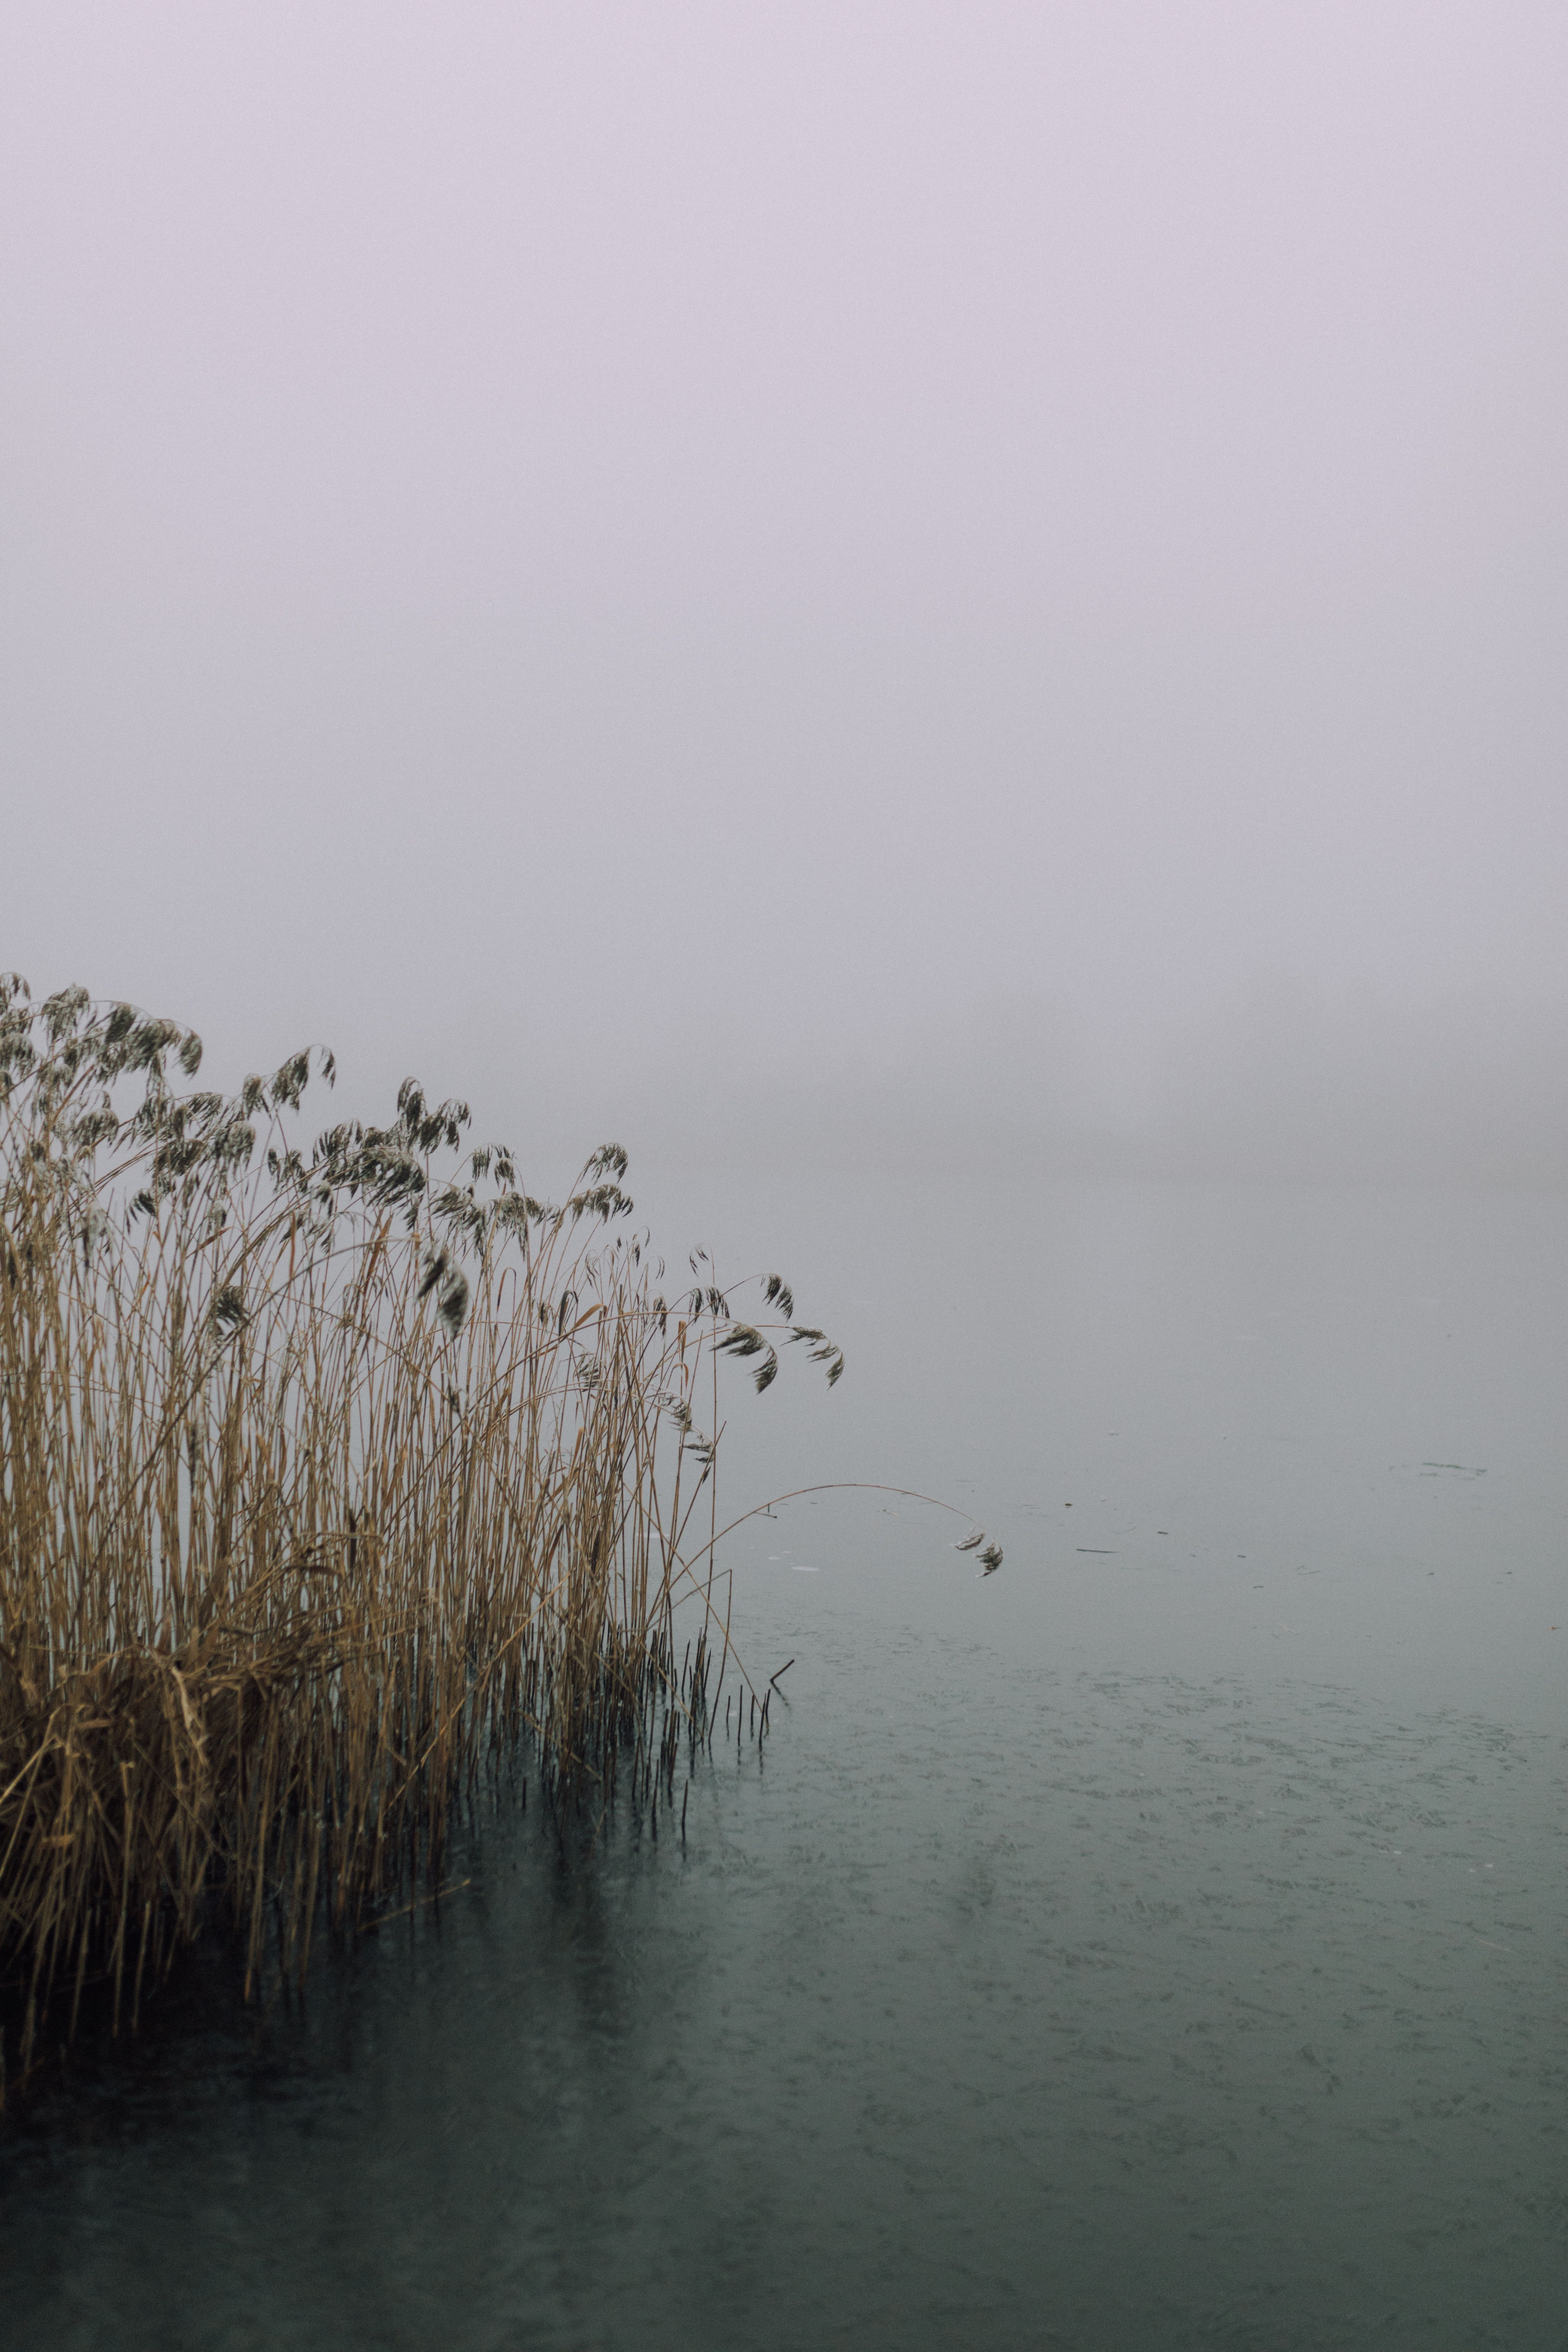
\includegraphics[width=.8\linewidth]{images/6.jpg}
        \caption{}
        \label{fig:life2}
    \end{subfigure}

    \begin{subfigure}{0.35\linewidth}
        \centering
        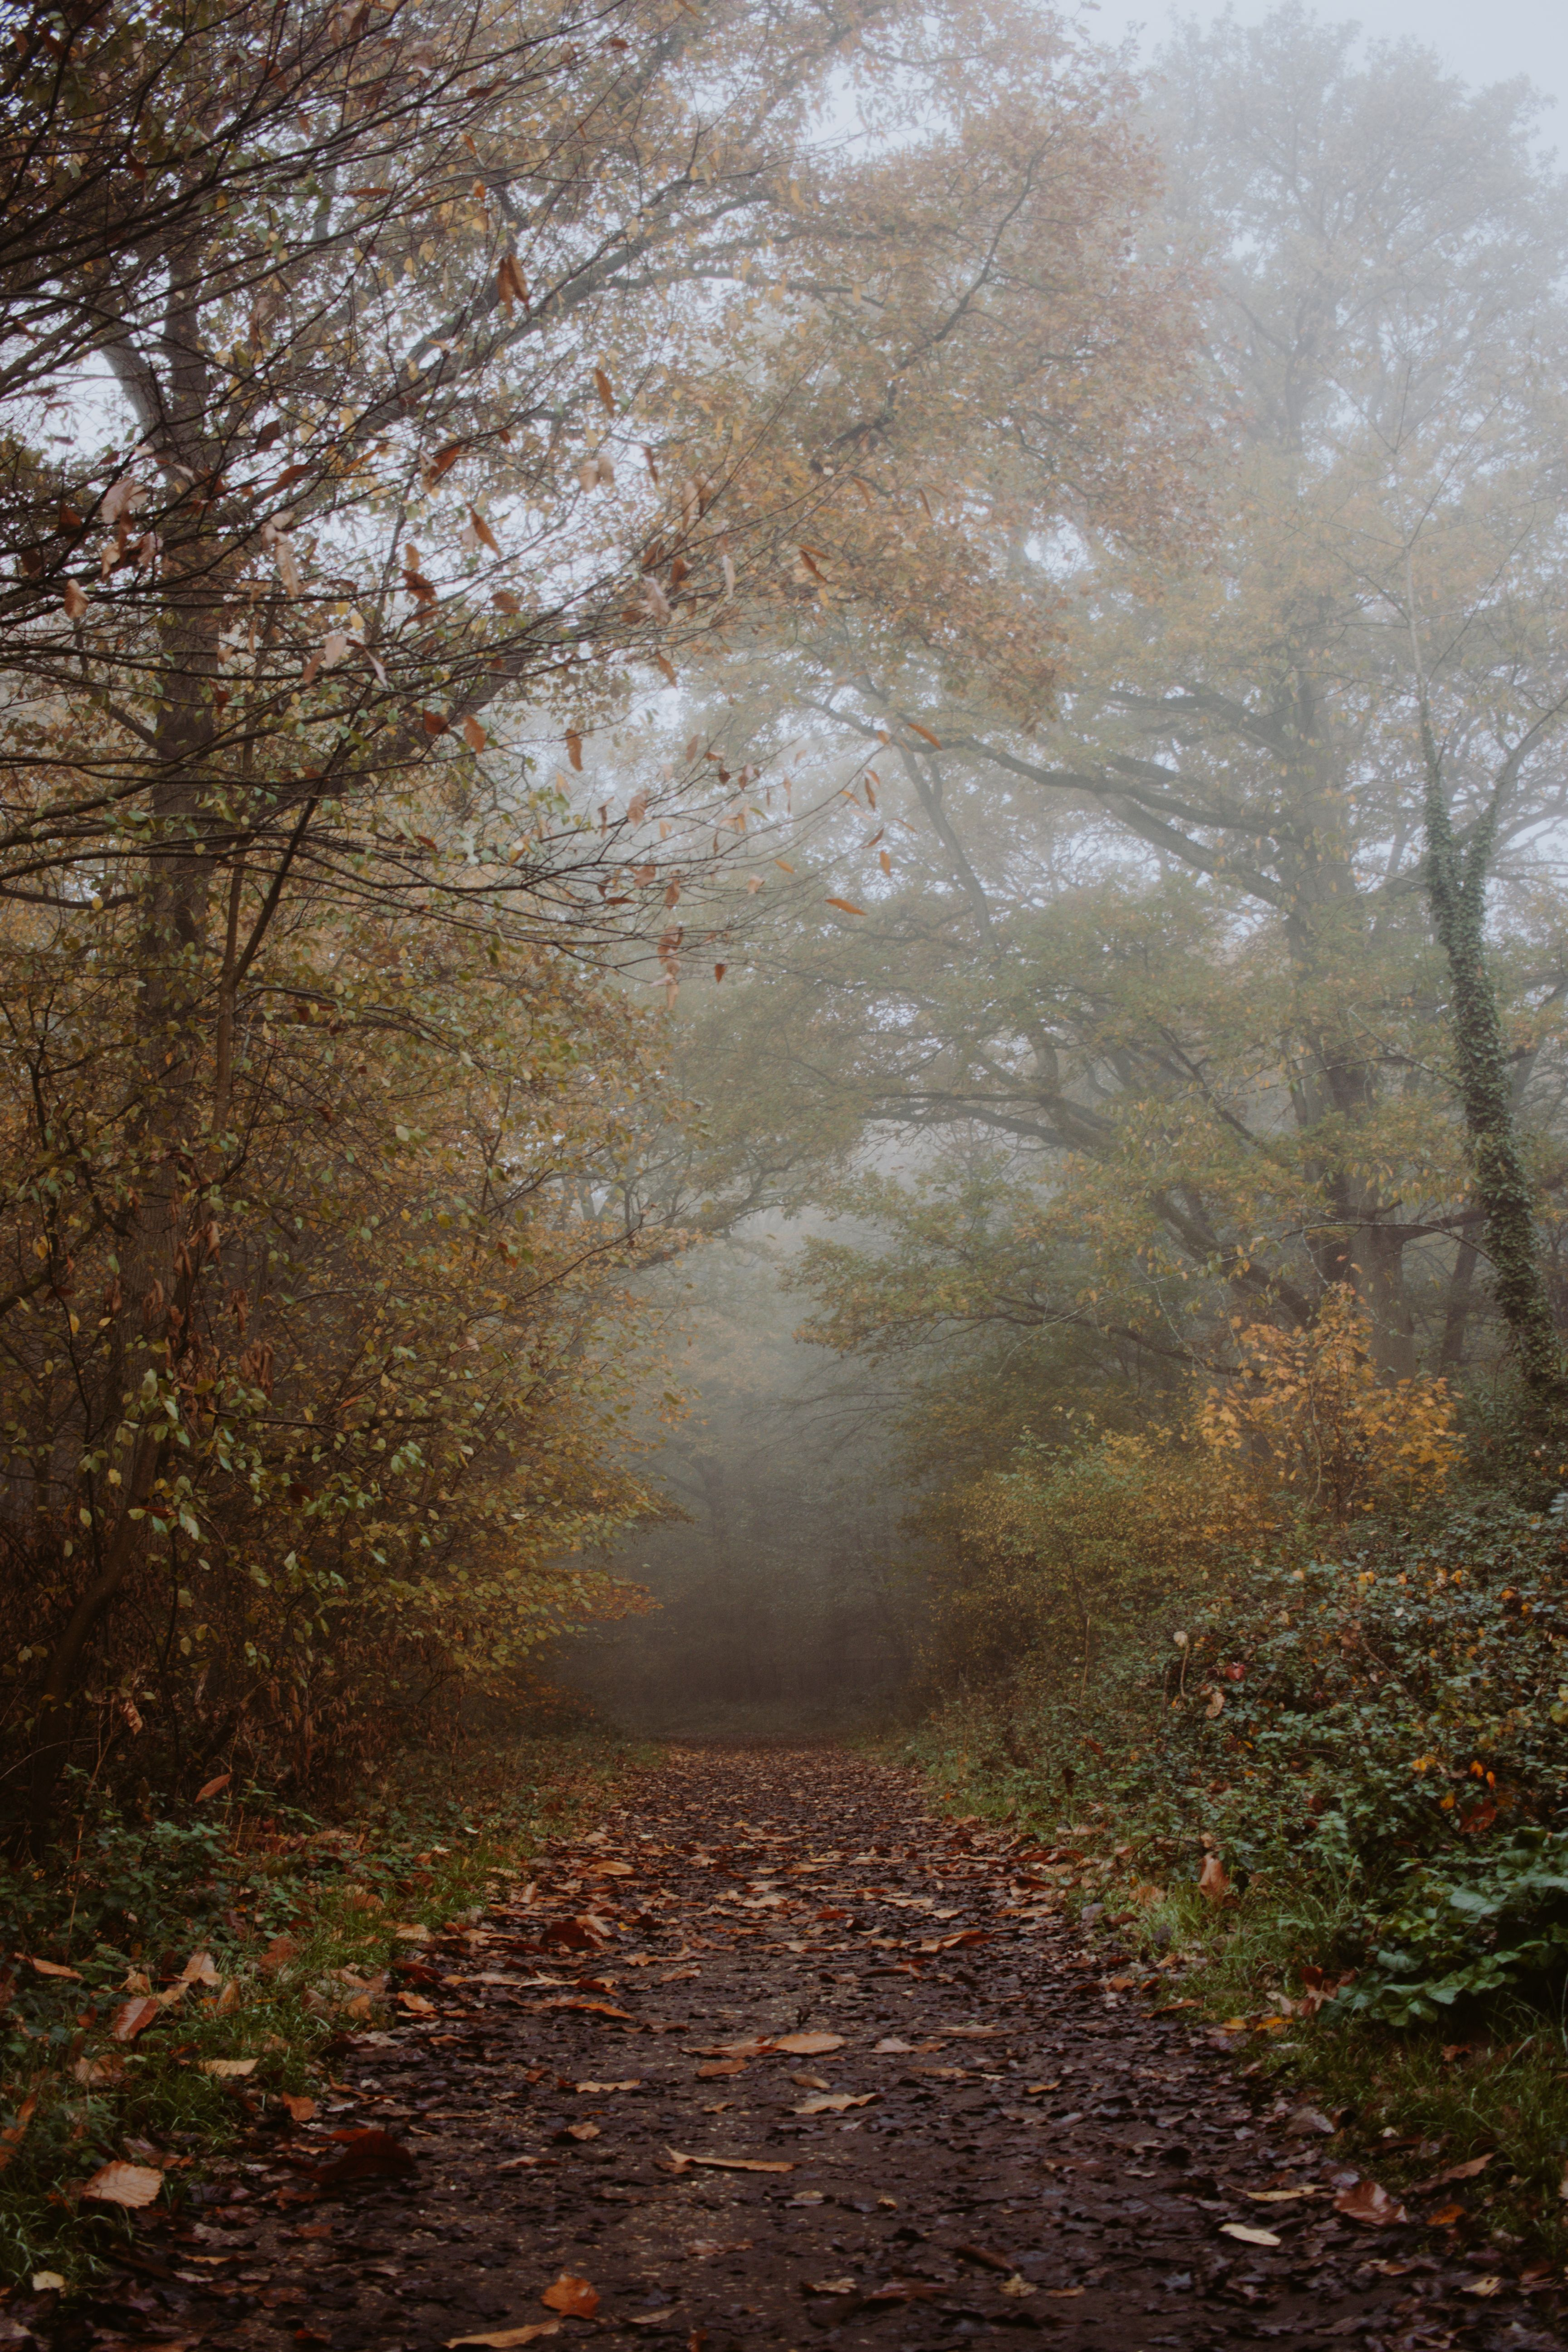
\includegraphics[width=.8\linewidth]{images/7.jpg}
        \caption{}
        \label{fig:life3}
    \end{subfigure}
    \hfill % Adds horizontal stretching space between the two images
    \begin{subfigure}{0.35\linewidth}
        \centering
        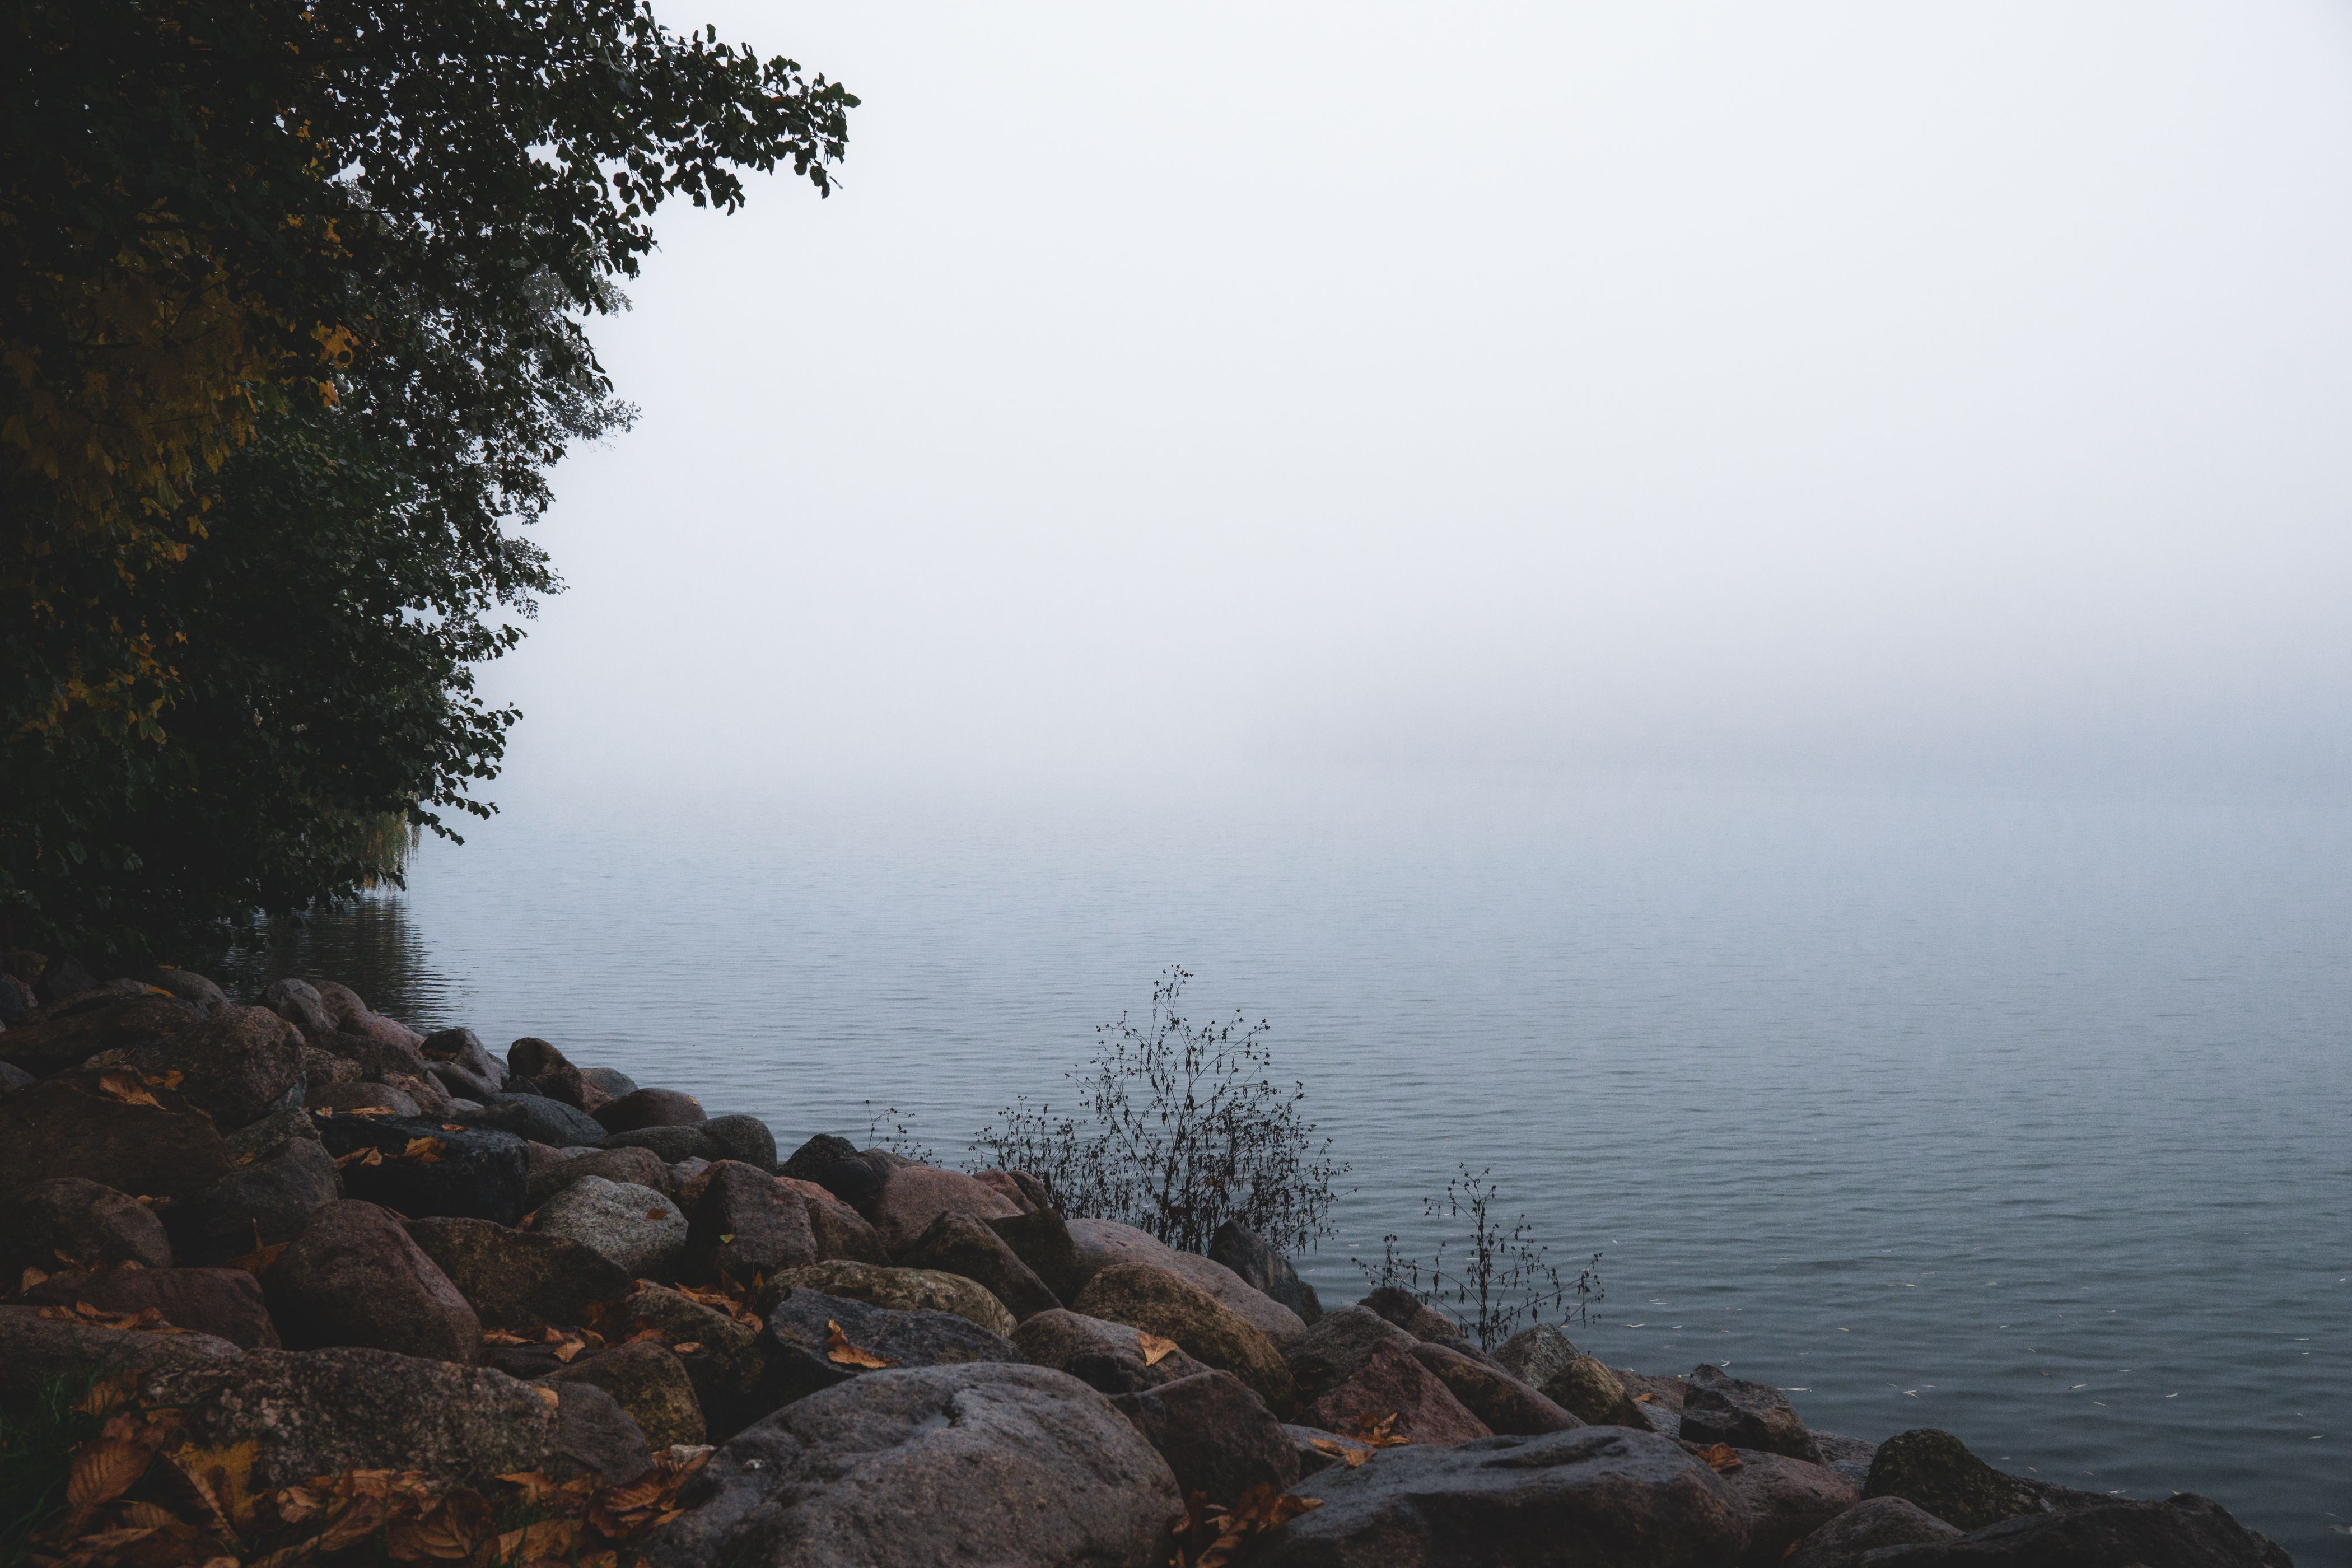
\includegraphics[width=.8\linewidth]{images/8.jpg}
        \caption{}
        \label{fig:life4}
    \end{subfigure}

    \caption{Four picture together}
\end{figure}

\lipsum[1-2]

\section{Hyperlink}

Visit \href{www.google.com}{Google} for searching paglami.
Here is the raw url \url{www.google.com}.

Here is a footnote \footnote{footnote example}

we can refer the Figure ~\ref{fig:life2} here.


\section{Citation example}

I am citing the work \cite{jarvis2014whole,vaswani2017attention}

\nocite{axfors2021association}   % list e rakhbe even though cite kora hoyni

\citet{vaswani2017attention} introduced transformer.

transformer was introduced in \citeyear{vaswani2017attention}.

\citeauthor{jarvis2014whole} introduced this.

\section{Algorithms}


\bibliographystyle{plainnat}
\bibliography{biblio}






\end{document}